% ---------------------------------------------------------------------------
% ---------------------------------------------------------------------------
% Junção de templates encontrados no Overleaf
% facilitando a vida do aluno de pós da UFABC
% Modelo LaTex para preparação do documento final de Dissertação de Mestrado
% ninguém do programa de pós da informação validou se presta
% ---------------------------------------------------------------------------
% ---------------------------------------------------------------------------

\documentclass[
	% -- opções da classe memoir --
	12pt,					% tamanho da fonte
	openright,				% capítulos começam em pág ímpar (insere página vazia caso preciso)
	twoside,					% para impressão em verso e anverso. Oposto a oneside
	a4paper,					% tamanho do papel. 
	% -- opções da classe abntex2 --
	%chapter=TITLE,			% títulos de capítulos convertidos em letras maiúsculas
	%section=TITLE,			% títulos de seções convertidos em letras maiúsculas
	%subsection=TITLE,		% títulos de subseções convertidos em letras maiúsculas
	%subsubsection=TITLE,	% títulos de subsubseções convertidos em letras maiúsculas
	% -- opções do pacote babel --
	english,					% idioma adicional para hifenização
	%french,					% idioma adicional para hifenização
	%spanish,				% idioma adicional para hifenização
	brazil					% o último idioma é o principal do documento
	]{abntex2}

% ---------------------
% Pacotes OBRIGATÓRIOS
% ---------------------
\usepackage{lmodern}				% Usa a fonte Latin Modern			
\usepackage[T1]{fontenc}			% Selecao de codigos de fonte.
\usepackage[utf8]{inputenc}		% Codificacao do documento (conversão automática dos acentos)
\usepackage{lastpage}			% Usado pela Ficha catalográfica
\usepackage{indentfirst}			% Indenta o primeiro parágrafo de cada seção.
\usepackage{color}				% Controle das cores
\usepackage{graphicx,graphicx}	% Inclusão de gráficos
\usepackage{epsfig,subfig}		% Inclusão de figuras
\usepackage{microtype} 			% Melhorias de justificação
% ---------------------
		
% ---------------------
% Pacotes ADICIONAIS
% ---------------------
\usepackage{lipsum}						% Geração de dummy text
\usepackage{amsmath,amssymb,mathrsfs}	% Comandos matemáticos avançados 
\usepackage{setspace}  					% Para permitir espaçamento simples, 1 1/2 e duplo
\usepackage{verbatim}					% Para poder usar o ambiente "comment"
\usepackage{tabularx} 					% Para poder ter tabelas com colunas de largura auto-ajustável
\usepackage{afterpage} 					% Para executar um comando depois do fim da página corrente
\usepackage{url} 						% Para formatar URLs (endereços da Web)
\usepackage{listings}					% para inserir trechos de código
\usepackage[raggedrightboxes]{ragged2e}
\usepackage{multirow}					% para tabelas com linhas 
% ---------------------

% ---------------------
% Pacotes de CITAÇÕES
% ---------------------
\usepackage[brazilian,hyperpageref]{backref}	% Paginas com as citações na bibl
\usepackage[alf]{abntex2cite}				% Citações padrão ABNT (alfa)
%\usepackage[num]{abntex2cite}				% Citações padrão ABNT (numericas)
% ---------------------

% ---------------------
% configuração das cores e dos trechos de código
% ---------------------
% \definecolor{azul}{rgb}{0,0,0.6}
% \definecolor{roxo}{rgb}{0.58,0,0.82}
% \definecolor{verde}{rgb}{0,0.6,0}

% \lstset{frame=tb,
%   language=yaml,
%   aboveskip=3mm,
%   belowskip=3mm,
%   showstringspaces=false,
%   columns=flexible,
%   basicstyle={\small\ttfamily},
%   numbers=none,
%   numberstyle=\tiny\color{roxo},
%   keywordstyle=\color{gree},
%   commentstyle=\color{dkgreen},
%   stringstyle=\color{mauve},
%   breaklines=true,
%   breakatwhitespace=true,
%   tabsize=3
% }

% ---------------------



% O tamanho da identação do parágrafo é dado por:
\setlength{\parindent}{1.3cm}

% Controle do espaçamento entre um parágrafo e outro:
\setlength{\parskip}{0.2cm}  % tente também \onelineskip


% ---------------------
% Compila o indice
% ---------------------
\makeindex
% ---------------------

% Configurações de CITAÇÕES para abntex2
% --- 
% CONFIGURAÇÕES DE PACOTES
% --- 

% ---
% Configurações do pacote backref
% Usado sem a opção hyperpageref de backref
\renewcommand{\backrefpagesname}{Citado na(s) página(s):~}
% Texto padrão antes do número das páginas
\renewcommand{\backref}{}
% Define os textos da citação
\renewcommand*{\backrefalt}[4]{
	\ifcase #1 %
		Nenhuma citação no texto.%
	\or
		Citado na página #2.%
	\else
		Citado #1 vezes nas páginas #2.%
	\fi}%
% ---

% Inclusão de dados para CAPA e FOLHA DE ROSTO (título, autor, orientador, etc.)
% ---
% Informações de dados para CAPA e FOLHA DE ROSTO
% ---
\titulo{Análise do desenvolvimento de uma inteligência artificial condutora de um veículo}
\autor{Vítor Guilherme Antunes}
\local{Santo André - SP}
\data{Dezembro de 2023}
\orientador{Fernando Teubl Ferreira}
% \coorientador{Fulano Nome do Coorientador}
\instituicao{%
  Universidade Federal do ABC -- UFABC
  \par
  Centro de Matemática, Computação e Cognição
  \par
  Projeto de Graduação em Computação}
\tipotrabalho{Dissertação (Mestrado)}
% O preambulo deve conter o tipo do trabalho, o objetivo,
% o nome da instituição e a área de concentração
\preambulo{\textbf{Projeto de Graduação} apresentada ao Centro de Matemática, Computação e Cognição, como parte dos requisitos necessários para a obtenção do Título de Bacharel em Ciência da Computação.}
% ---

% Inclui Configurações de aparência do PDF Final
%  Configurações de aparência do PDF final
% NÃO ALTERAR!!!

% alterando o aspecto da cor azul
\definecolor{blue}{RGB}{41,5,195}

% informações do PDF
\makeatletter
\hypersetup{
     	%pagebackref=true,
		pdftitle={\@title}, 
		pdfauthor={\@author},
    		pdfsubject={\imprimirpreambulo},
	    pdfcreator={LaTeX with abnTeX2},
		pdfkeywords={abnt}{latex}{abntex}{abntex2}{trabalho acadêmico}, 
		colorlinks=true,       		% false: boxed links; true: colored links
    		linkcolor=blue,          	% color of internal links
    		citecolor=blue,        		% color of links to bibliography
    		filecolor=magenta,      		% color of file links
		urlcolor=blue,
		bookmarksdepth=4
} 
\makeatother
% --- 

%%%%%%%%%%%%%%%%%%%%%%%%%%%
%%  INICIO DO DOCUMENTO  %%
%%%%%%%%%%%%%%%%%%%%%%%%%%%
\begin{document}

% Retira espaço extra obsoleto entre as frases.
\frenchspacing

% ----------------------------------------------------------
% ELEMENTOS PRÉ-TEXTUAIS (Capa, Resumo, Abstract, etc.)
% ----------------------------------------------------------
\pretextual

% Capa
% ---
% Impressão da Capa
% ---
  \begin{capa}%
    \begin{figure}[h!]%
        \centering%
        
\includegraphics[scale=1.2]{figs/logo.png}%
    \end{figure}%
    \center
	\ABNTEXchapterfont\large{Universidade Federal do ABC \\ Centro de Matemática, Computação e Cognição \\ Projeto de Graduação em Computação}
	%\vspace{1.5cm}

    \vfill
    \ABNTEXchapterfont\bfseries\LARGE\imprimirtitulo
    \vfill

	%\vfill
	\ABNTEXchapterfont\large\imprimirautor
	\vfill
%
	% Número de Ordem : XXXX
	
    \large\imprimirlocal, \large\imprimirdata

    \vspace*{1cm}
  \end{capa}
% ---

% Folha de rosto (o * indica que haverá a ficha bibliográfica)
\imprimirfolhaderosto*

% Imprimir Ficha Catalografica
% ---
% Ficha Catalográfica
% ---
% Isto é um exemplo de Ficha Catalográfica, ou ``Dados internacionais de
% catalogação-na-publicação''. Você pode utilizar este modelo como referência. 
% Porém, talvez a biblioteca lhe fornece um PDF
% com a ficha catalográfica definitiva após a defesa do trabalho. Quando estiver
% com o documento, salve-o como PDF no diretório do seu projeto e substitua todo
% o conteúdo de implementação deste arquivo pelo comando abaixo:
%
% \begin{fichacatalografica}
%     \includepdf{fig_ficha_catalografica.pdf}
% \end{fichacatalografica}
\begin{fichacatalografica}
	\vspace*{\fill}					% Posição vertical
	\hrule							% Linha horizontal
	\begin{center}					% Minipage Centralizado
	\begin{minipage}[c]{12.5cm}		% Largura
	
	\imprimirautor
	
	\hspace{0.5cm} \imprimirtitulo  / \imprimirautor. --
	\imprimirlocal, \imprimirdata-
	
	\hspace{0.5cm} \pageref{LastPage} p. : il. (algumas color.) ; 30 cm.\\
	
	\hspace{0.5cm} \imprimirorientadorRotulo~\imprimirorientador\\
	
	\hspace{0.5cm}
	\parbox[t]{\textwidth}{\imprimirtipotrabalho~--~\imprimirinstituicao,
	\imprimirdata.}\\
	
	\hspace{0.5cm}
		1. Palavra-chave1.
		2. Palavra-chave2.
		I. Orientador.
		II. Universidade xxx.
		III. Faculdade de xxx.
		IV. Título\\ 			
	
	\hspace{8.75cm} CDU 02:141:005.7\\
	
	\end{minipage}
	\end{center}
	\hrule
\end{fichacatalografica}
% ---

% Inserir Folha de Aprovação
% % ---
% Assinaturas
% ---
% Isto é um exemplo de Folha de aprovação, elemento obrigatório da NBR
% 14724/2011 (seção 4.2.1.3). Você pode utilizar este modelo até a aprovação
% do trabalho. Após isso, substitua todo o conteúdo deste arquivo por uma
% imagem da página assinada pela banca com o comando abaixo:
%
% \includepdf{folhadeaprovacao_final.pdf}
%
\begin{folhadeaprovacao}

  \begin{center}
    {\ABNTEXchapterfont\large\imprimirautor}

    \vspace*{\fill}\vspace*{\fill}
    \begin{center}
      \ABNTEXchapterfont\bfseries\Large\imprimirtitulo
    \end{center}
    \vspace*{\fill}
    
    \hspace{.45\textwidth}
    \begin{minipage}{.5\textwidth}
        \imprimirpreambulo
    \end{minipage}%
    \vspace*{\fill}
   \end{center}
        
 % Isso na versao final do trabalho!!!       
   Trabalho aprovado. \imprimirlocal, 01 de janeiro de 2014:

   \assinatura{\textbf{\imprimirorientador} \\ Orientador} 
   \assinatura{\textbf{\imprimircoorientador} \\ Co-Orientador} 
   \assinatura{\textbf{Professor} \\ Convidado 1}
   \assinatura{\textbf{Professor} \\ Convidado 2}
   \assinatura{\textbf{Professor} \\ Convidado 3}
      
   \begin{center}
    \vspace*{0.5cm}
    {\large\imprimirlocal}
    \par
    {\large\imprimirdata}
    \vspace*{1cm}
  \end{center}
  
\end{folhadeaprovacao}
% ---

% Dedicatória
% % ---
% Dedicatória
% ---
\begin{dedicatoria}
   \vspace*{\fill}
   \centering
   \noindent
   \textit{ Aos verme que roeu as frias carnes de meu cadáver.} \vspace*{\fill}
\end{dedicatoria}
% ---

% Agradecimentos
% ---
% Agradecimentos
% ---
\begin{agradecimentos}

Agradeço primeiramente a minha família, por sempre me apoiarem e motivarem nos estudos.

Agradeço ao meu orientador, Fernando Teubl, por ter me acompanhado durante a realização deste trabalho.

Aos meus colegas e amigos que fiz durante a minha graduação na UFABC, que contribuiram bastante pro meu desempenho acadêmico e profissional.

\end{agradecimentos}
%% ---

% Epígrafe
% ---
% Epígrafe
% ---
\begin{epigrafe}
    \vspace*{\fill}
	\begin{flushright}
		\textit{``Não sei o que, \\
		          não sei o que,\\
                  não sei o que lá.''\\
		          (Autor Desconhecido)}
	\end{flushright}
\end{epigrafe}
% ---

% Resumo e Abstract
% ---
% RESUMOS
% ---

% RESUMO em português
\setlength{\absparsep}{18pt} % ajusta o espaçamento dos parágrafos do resumo
\begin{resumo}
Veículos autônomos são um dos grandes objetivos da indústria automotiva atualmente, embora muito progresso já foi feito e testes nas ruas já são uma realidade, muitos desafios éticos estão no caminho para o aperfeiçoamento da tecnologia, por exemplo, como o veículo reagiria em caso de vida ou morte. Com isso em mente, este projeto se propõe de criar um simulador utilizando da Unity3D, uma game engine, para o treinamento de veículos autônomos, e que sirva de plataforma para estudos futuros podendo criar diversos cenários hipotéticos. Neste projeto, pretende fazer estudos comparativos de algoritmos de aprendizado por reforço e aprendizado por imitação no ambiente do simulador recém-criado.

 \textbf{Palavras-chaves}: Veículos autônomos. Aprendizado por Reforço. Aprendizado por Imitação.
\end{resumo}

% ABSTRACT in english
\begin{resumo}[Abstract]
 \begin{otherlanguage*}{english}
   Autonomous vehicles are one of the biggest goals of the automotive industry nowadays, although a lot of progress have been made and tests on road are already a thing, many ethical challenges are in the way of enhancement of this technology, such as how an autonomous vehicle would react in a life or death situation. With this in mind, this project aims to build a simulator using Unity3D game engine for the training of agents capable of driving a vehicle, which can be used as a platform for future studies around hypothetical scenarios. In this project, we intend to do early comparative studies about Reinforcement Learning and Imitation Learning algorithms in the newly developed simulation environment.

   \vspace{\onelineskip}
 
   \noindent 
   \textbf{Keywords}: Autonomous Vehicles. Reinforcement Learning. Imitation Learning.
 \end{otherlanguage*}
\end{resumo}

% Lista de ilustrações
\pdfbookmark[0]{\listfigurename}{lof}
\listoffigures*
\cleardoublepage

% Lista de tabelas
\pdfbookmark[0]{\listtablename}{lot}
\listoftables*
\cleardoublepage

% Lista de abreviaturas e siglas
\begin{siglas}
  \item[IA] Inteligência Artificial
  \item[AS] Aprendizado Supervisionado
  \item[MDP] Processo de Decisão de Markov
  \item[PGM] Policy Gradient Method (Método de polítca gradiente)
  \item[PPO] Proximal Policy Optimization
  \item[SAC] Soft Actor Critic
  \item[IRL] Inverse Reinforcement Learning
  \item[BC]  Behavioural Cloning
  \item[GAIL] Generative Adversarial Imitation Learning
\end{siglas}

% Lista de símbolos
\begin{simbolos}
	\item[$ \in $] Pertence
	\item[$ \doteq $] Se define por
	\item[$ S $] Conjunto de estados
	\item[$ S^+ $] Conjunto de estados onde há estado terminal
	\item[$ A $] Conjunto de ações
	\item[$ A(s) $] Conjunto de ações válidas no estado $s$
	\item[$ \pi $] Política
	\item[$ \pi_\ast $] Política ótima
	\item[$ v(s) $] função valor do estado s
	\item[$ v_\pi(s) $] função valor do estado s sob política $\pi$
	\item[$ q(s,a) $] função valor do ação-estado
	\item[$ q_\pi(s,a) $] função valor do ação-estado sob política $\pi$
	\item[$ \gamma $] Constante de desconto
\end{simbolos}

% Inserir o SUMÁRIOAdversarial
\pdfbookmark[0]{\contentsname}{toc}
\tableofcontents*
\cleardoublepage

% ----------------------------------------------------------
% ELEMENTOS TEXTUAIS (Capítulos)
% ----------------------------------------------------------
\textual
% Elementos textuais com numeração arábica
\pagenumbering{arabic}
% Reinicia a contagem do número de páginas
\setcounter{page}{1}

% Inclui cada capitulo da Dissertação
% ----------------------------------------------------------
% Introdução 
% Capítulo sem numeração, mas presente no Sumário
% ----------------------------------------------------------

\chapter*[Introdução]{Introdução}
\addcontentsline{toc}{chapter}{Introdução}

No passado eram veículos eram, em grande parte, máquinas mecânicas, com poucos recursos eletrônicos. Hoje em dia, diversos avanços foram feitos nos carros modernos, e estes já estão equipados com variadas tecnologias assistentes como controle de tração, freios ABS e de emergência, piloto automático, entre outros recursos que dependem de sensores e que tomam decisões que controlam parcialmente o veículo, visando segurança e conforto ao condutor. 

Veículos que possuem as assistências mencionadas acima comumente são chamados de "autônomos", porém neste artigo trataremos por "carro autônomo" um veículo que seja capaz de conduzir-se sem depender de um humano. De acordo com o padrão SAE J3016 a autonomia de veicular é dividida em níveis que vão do zero ao cinco, os recursos citados são no máximo nível 2, um veículo para ser "autônomo" seria de nível 3 ou maior (\citeonline{SAE2014}), porém para atingir este grau de autonomia é necessário mais do que sensores e controladores que dão instruções diretas ao carro.

\begin{comment}
Inserir aqui um parágrafo sobre o estado atual dos carros autônomos na indústria e no mercado
\end{comment}

Nas duas últimas décadas houve um aumento na presença de tecnologias como Inteligência Artificial e \textbf{Aprendizado de Máquina} no cotidiano das pessoas. Corretores ortográficos, reconhecimento facial, algoritmos de recomendação de leitura, música ou compra são alguns exemplos de diversos outros que até então estavam apenas disponíveis em lugares específicos com laboratórios de pesquisa, mas agora já são amplamente aplicadas. 

Existem três paradigmas de aprendizado de máquina: \textbf{aprendizado supervisionado}, \textbf{não supervisionado} e \textbf{aprendizado por reforço}. Este último aborda aprendizado que envolvam exercer uma atividade, nele, o \textbf{agente} durante seu treino, aprimora uma tarefa após várias tentativas e erro onde é premiado quando age corretamente e penalizado caso contrário. Este artigo introduzirá os dois primeiros paradigmas e discorrerá mais detalhadamente sobre o \textbf{AR}. Embora o \textbf{AS} também é necessário para a tarefa, ele é mais usado em reconhecimento de elementos no ambiente, algo que está fora do escopo deste projeto.

Quando tenta-se criar uma automato que exerça uma atividade complexa como condução de um veículo, a abordagem clássica que usa algoritmos com condicionais e instruções direta é insuficiente para tal, isto deve-se ao fato de que é inviável criar manualmente uma tabela de comandos dado certas condições, a lista tenderia ao infinito. Utilizando de um paradigma de AM como \textbf{aprendizado por reforço} se faz necessário pois o automato irá, após sucessivas tentativas, dominar a técnica de conduzir um veículo.

\begin{comment}
    Introduzir brevemente o PPO e SAC aqui
\end{comment}

Este artigo propõe-se a apresentar um estudo do que é necessário para criar um agente condutor de um veículo dentro de um simulador que saiba percorrer um dado trajeto em um ambiente urbano. Será analisado como modelar um simulador, como quais sensores o veículo deve possuir, quais observações deve fazer do ambiente para evitar colisões, entre outros.


\section*{Justificativa}\label{sec:justificativa}
\addcontentsline{toc}{section}{Justificativa}
Uma das maiores causas de morte no Brasil é por conta de acidentes de trânsito, chegando a um total de 43 mil óbitos em um único ano (CARVALHO, 2016), é sabido também que grande causa dessas mortes é por falha humana por parte do condutor. Tendo em vista o avanço tecnológico na área de Inteligência Artificial vemos que vem se tornando viável o desenvolvimento de um modelo que seja capaz de conduzir um veículo automotivo em ambientes urbanos, dessa forma poderíamos ter em vias públicas condutores que não se distraiam e não cometam infrações de trânsitos.


\section*{Objetivos}\label{sec:objetivos}
\addcontentsline{toc}{section}{Objetivos}
O objetivo deste projeto é criar uma simulação que se aproxime o máximo possível a um cenário real e com isso analisar todos os elementos que são necessários para que o agente aprende a exercer sua tarefa mais central: conduzir o veículo de sua origem até seu destino.
\begin{itemize}
    \item Analisar quantos sensores o veículo deve possuir, como devem ser posicionados. 
    \item Como a adição gradual de cada elemento de trânsito afeta o agente (elementos como outros veículos, semáforos e pedestres)
    \item Diferença entre os algoritmos de otimização de política \textbf{SAC} e \textbf{PPO} afetam a convergência do treino e o resultado final
\end{itemize}

\section*{Etapas do estudo}\label{sec:etapas}
\addcontentsline{toc}{section}{Etapas do estudo}
Podemos abstrair o treino em três segmentos: \textbf{ambiente}, \textbf{agente} e \textbf{algoritmo}. Ambiente engloba qualquer coisa que o agente interage, por exemplo, o cenário urbano como as ruas e calçadas, e uma inclusão de elementos de trânsito como outros veículos, semáforos ou pedestres seriam alterações no ambiente. O segundo segmento se refere ao aprendiz, alterações feitas nas informações recebidas pelo agente como distância dos obstáculos mais próximos, velocidade do veículo, distância e localização do destino, etc, mudanças feitas nestas propriedades ou em semelhantes são alterações no agente. Finalmente, algoritmo se refere ao esquema dos algoritmos usados (PPO ou SAC) e seus hiper-parâmetros.

A primeira etapa deste estudo o agente terá de aprender a conduzir como se estivesse sozinho, isso permitirá entender melhor o que é necessário para fazer com que o aprendiz precisa para percorrer qualquer trajeto dado como objetivo. Isto é o ambiente inicialmente será apenas uma cidade vazia e a cada etapa deve-se aumentar a complexidade dele visando se aproximar da realidade. Em cada etapa as mudanças devem seguir a ordem dos segmentos, com uma certa flexibilidade, ou seja, um aumento de realismo no ambiente deve levar a alterações sensoriais no agente para se adaptar ao novo cenário e calibrar os hiper-parâmetros dos algoritmos usados.

Em cada etapa então deve-se:
\begin{itemize}
    \item Analisar quantos e como serão dispostos os sensores o veículo deve possuir;
    \item Como é o desempenho usando cada algoritmo (PPO ou SAC), como as alterações dos hiper-parâmetros afetam o treino e a convergência/otimização do comportamento;
\end{itemize}

% PARTE - Define a divisão do documento em partes (Não é obrigatório)
\part{Preparação da pesquisa}
% ---
\chapter{Fundamentação teórica}
% ---
Neste capítulo será introduzido os conceitos e fundamentos das teorias e tecnologias utilizadas neste projeto. Será abordado os paradigmas de aprendizado de máquina com foco em aprendizado por reforço. Também abordará sobre autonomia de veículos como o que define um carro autônomo e os diferentes níveis de autonomia. Por fim, o que é um motor de jogo e a principal ferramenta que usaremos para desenvolver um ambiente simulado, a Unity 3D.

\section{Veículos autônomos}
A SAE (Society of Automotive Engineers) define 6 níveis de autonomia para veículos, do zero ao cinco (\citeonline{SAE2014}). O primeiro, nível zero, não possui automação de direção alguma, é limitado a apenas a tecnologias de assistência como freios ABS ou freio automático emergencial. Um veículo com automação de nível um já passa a possuir alguns recursos que ajudam na direção, como controle para manter o carro na via, controle de velocidade a fim de manter distância de outro veículo a frente. Os níveis dois e três são definidos por, respectivamente, "direção parcialmente automática" e "direção automática condicional", a diferença de ambos pode ser bem sútil, pois em ambos os casos a automação teria o controle do volante, acelerador e freio, no primeiro seria apenas para atividades mais simples, como dirigir na estrada mantendo a velocidade e distâncias, enquanto no nível três o veículo assumiria o controle por um período, podendo até fazer manobras mais avançadas, como ultrapassar um automóvel mais lento a frente. Em ambos os níveis ainda é necessário a atenção máxima do condutor para assumir o controle quando for necessário.

Nos últimos dois níveis de autonomia, temos um veículo que seria capaz de exercer qualquer atividade sem intervenção humana, no nível 4 não seria necessário que o motorista estivesse a condução, só assumiria o controle quando necessário, nesses níveis é capaz inclusive que o automóvel assuma o controle quando necessário, e o mesmo poderia ainda nem possuir volante ou pedais.

Atualmente veículos com autonomia de nível zero a dois, já estão presentes no mercado, nesse artigo estamos interessados em discutir sobre os carros autônomos de nível 3 ou mais, isto é, automóveis que possuam um alto nível de autonomia, o sistema deles podem ser divididos em quatro componentes, cada um deles usam aprendizado de máquina de formas diferentes, são eles: planejamento de rota, decisões comportamentais, controle de moção e controle veicular (\citeonline{Paden2016}). 

O planejamento de rota se trata de definir o trajeto a ser percorrido pelo veículo, isto é, o cálculo do percurso da origem ao destino, imaginar uma cidade com suas ruas, intersecções e pontos de destino como se fosse um grafo ponderado com arestas e vértices e aplicar um algoritmo de busca como Djikstra não é o suficiente para gerar uma solução eficiente, então para isso requer algo que se utilize de outros dados como informação histórica e em tempo real para achar o melhor caminho a ser percorrido em um dado dia da semana, em um dado horário e clima.

Definida a rota, o veículo deve ser capaz de percorrer a mesma tendo em consideração todos os participantes do tráfego e as regras de trânsito, isso envolve uma complexidade de comportamento que vai além de apenas saber conduzir o veículo, então o componente de decisões comportamentais deve saber selecionar ações apropriadas para cada situação. A condução do automóvel em uma rodovia é diferente da condução em um cruzamento em uma rua urbana, onde ele deve parar o veículo e cruzar quando não há nenhum outro veículo ou pedestre no caminho.

A partir do momento que o comportamento foi selecionado, o controle de moção do automóvel autônomo que decide como este vai se locomover, mudança de faixa, conversão a direita, parar o veículo, avançar ao sinal verde, etc, todos essas ações devem ser realizadas de modo que não cause colisões, evitando obstáculos, e devem de ser realizada de forma que não cause desconforto aos passageiros.

O controle do veículo se define pelo controle dos atuadores mecânicos do automóvel para que tenha uma resposta em retorno, essa constante troca de informação é necessária para o controle de moção do veículo atue apropriadamente.

\section{Motores de jogos}
Um motor de jogo (do inglês \textit{game engine}) é um \textit{software} com o objetivo primário de se criar jogos eletrônicos. Estes programas inclui diversas ferramentas que auxiliam o desenvolvedor de jogos a criar seu produto, não existe uma definição sobre quais destas um software deve possuir para ser considerado um motor de jogo, mas frequentemente possuem módulos que lidam com \textit{input} de usuário, renderização de gráficos 2D e 3D, som, motor de física (onde se lida com gravidade e colisão), animação, gerenciamento de memória entre outros (\citeonline{Andrade2015}). 

% Considerar escrever um pouco sobre outros usos de uma game engine aqui, talvez seja necessário para fortalecer o argumento que uma game engine pode ser usada para um simulador e não apenas jogos podendo ter um uso mais "sério"

Como o objetivo é focado no desenvolvimento de uma inteligência artificial para um simulador de carro autônomo, um motor de jogo possui meios que facilitariam o trabalho, não seria necessário desenvolver do zero a renderização dos modelos dos ambientes como veículos, ruas, calçadas, prédios, etc, também não seria necessário desenvolver todo o complexo cálculo de física como força, gravidade, colisão de objetos, peso do veículo, entre outros. Com isso permite que o foco do trabalho a ser feito se limite o máximo possível à análise da IA.

Inicialmente foi considerado o uso de outros motores de jogo, como a Unreal Engine 4 (software da Epic Games, Inc.) e a Godot Engine (Open Source sob licença MIT), embora haja uma preferência natural por uma ferramenta open source do que um software proprietário para realizar esta tarefa, a Unity 3D possui uma comunidade muito maior que o Godot Engine de acordo com (\citeonline{ITCHIO2023}) e (\citeonline{STEAMDB2023}), ambas as fontes são portais que servem para divulgação e venda de jogos publicados por desenvolvedores individuais ou empresas, a Unity 3D é mais utilizada em ambas as plataformas. A Unity 3D possui também seu acervo de recursos criados pela comunidade conhecido como Unity Asset Store onde é possível obter modelos 3D, efeitos sonoros e até modelos genéricos de jogos para se construir algo em cima disso. 

A Unity 3D também possui uma biblioteca de ferramentas própria para criação de agentes inteligentes chamada de \textbf{Unity ML Agent Toolkit}, que foi escrita usando \textbf{Pytorch}, uma biblioteca \textbf{Python} para criação de redes neurais. A Unity ML Agent toolkit oferece um aparato para se criar um agente inteligente, onde é configurado sensores e ações (o que seria a primeira e última camada de uma rede neural) podendo ser treinado usando aprendizado por reforço, por imitação, neuroevolução, entre outros.

\subsection{Editor da Unity3D}
Dentre as principais janelas da interface da Unity3D, temos: hierarquia, projeto, visualização da cena e inspetor. A primeira se trata dos elementos que há dentro da cena (pode-se entender como sendo um trecho do jogo, como este projeto contém apenas uma única cena não é necessário que o leitor entenda tudo que uma cena pode ser), estes elementos são chamados de \textit{GameObjects}, eles são uma abstração de qualquer item dentro do jogo, incluindo o personagem que o jogador controla, o cenário com o qual interage, a "câmera" com o qual o jogo é visto também é um \textit{GameObject}. A primeira janela é chamada de hierarquia porque o conjunto destes objetos podem formar uma estrutura em árvore, por exemplo, podemos criar um objeto "árvore" que conteria os objetos "raiz", "tronco" e "folhas" como seus objetos aninhados. Na seção da proposta é explicado a estrutura deste projeto com mais detalhes.

\begin{figure}[h]
   \centering
   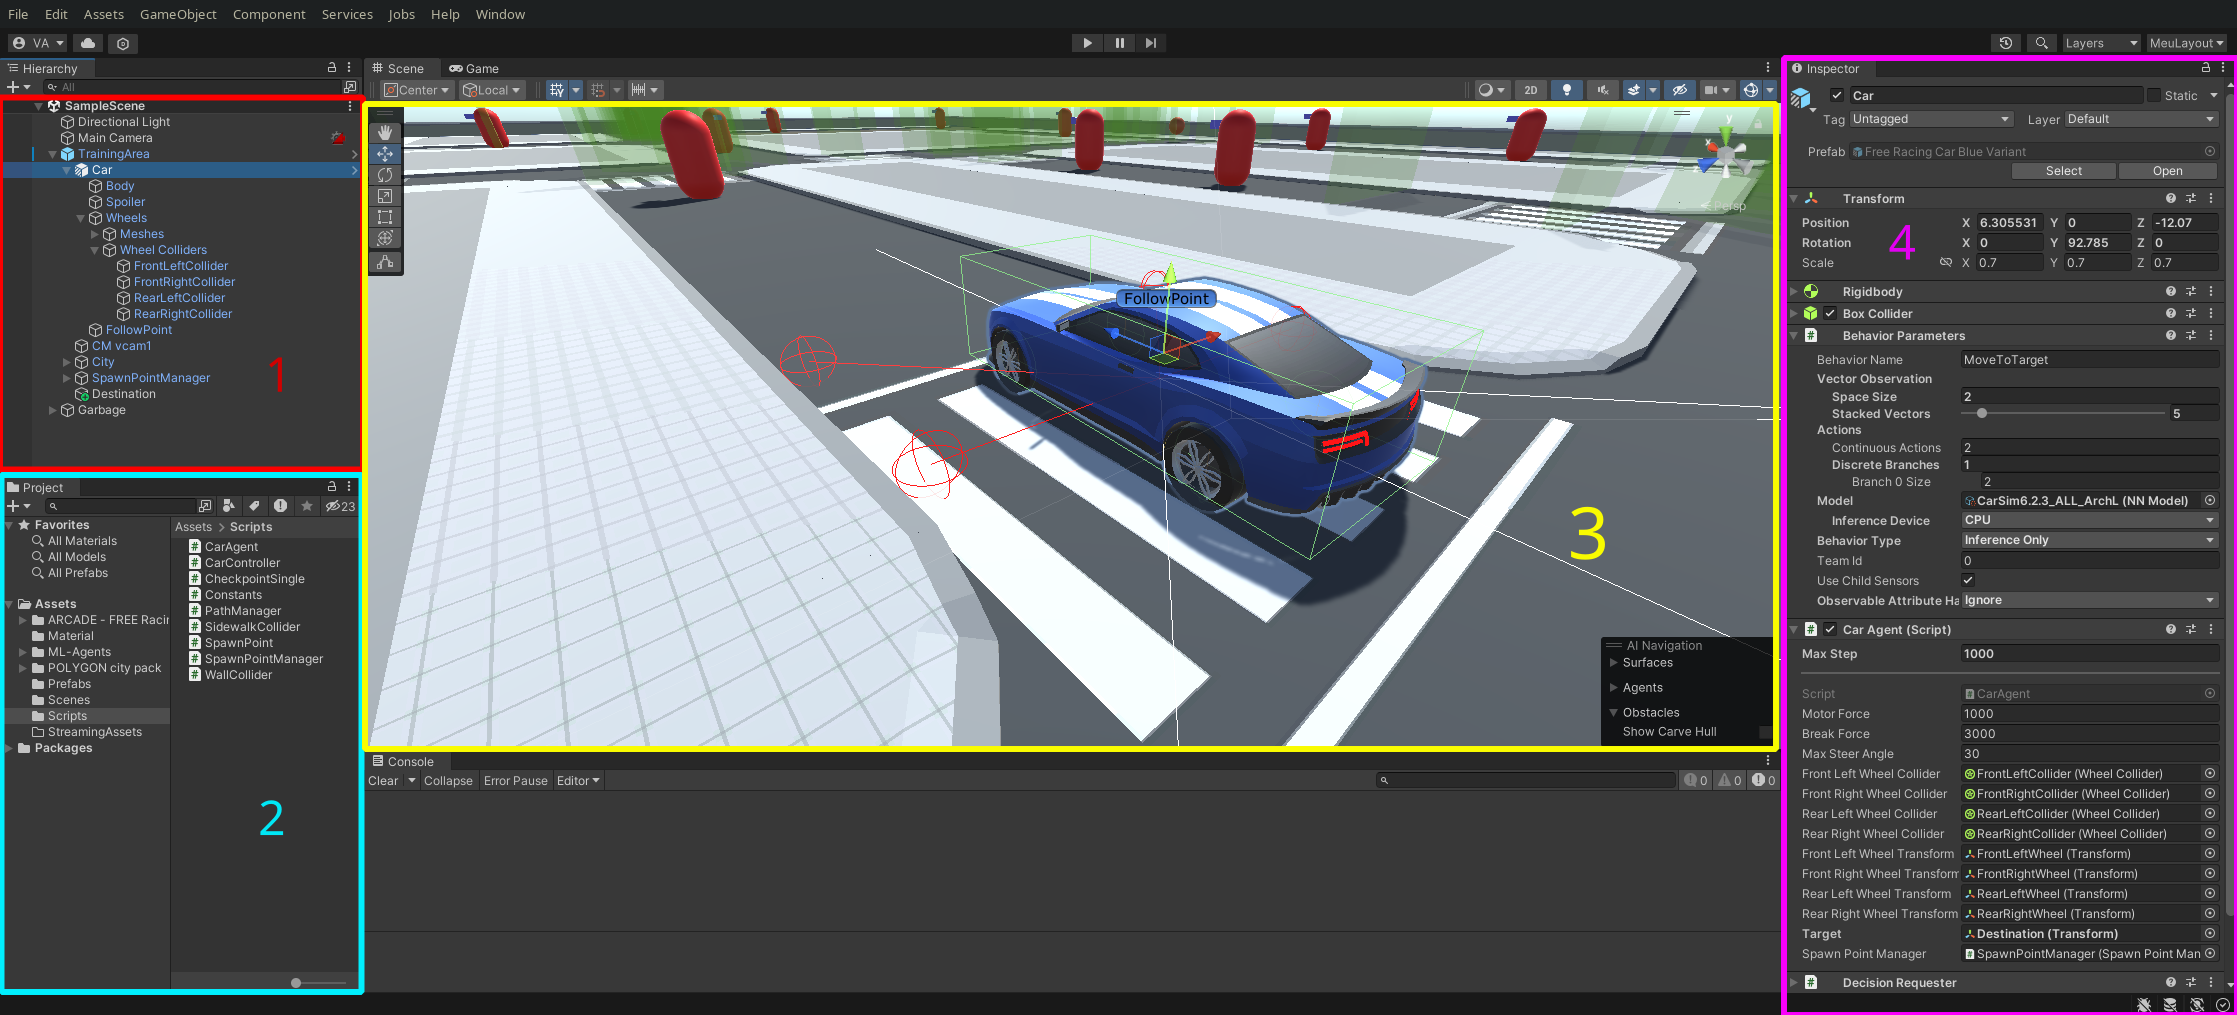
\includegraphics[scale=0.2]{figs/interface-unity3d-indicadores.png}
    \caption{Interface da Unity3D. A janela 1 é a hierarquia, 2 é a janela de projeto, 3 é visualização da cena e 4 é o inspetor}
    \label{fig:prefixt}
 \end{figure}

A janela de projeto estão os arquivos do projeto, é um diretório do projeto criado pela Unity3D onde deve conter arquivos de efeitos sonoros, códigos-fonte do desenvolvedor, fontes, modelos 2D e 3D, texturas, etc. A visualização da cena é uma janela que permite o desenvolvedor ter uma noção visual da disposição dos \textit{GameObjects}, desta forma ele consegue posicioná-los mais apropriadamente, também consegue ver se a dimensão e escala deles estão coerentes. 

A última janela é o inspetor, nela é exibido os detalhes dos \textit{GameObjects}, isto é, os \textit{components} destes. Como foi explicado anteriormente, os \textit{GameObjects} podem assumir diversas funcionalidades, e são os componentes que permitem isso, por exemplo, o componente \textit{Transform}, comum a todos os objetos da cena define as coordenadas (ou posição) que o objeto se encontrará na cena, sua rotação e escala, já os \textit{components} \textit{Mesh Filter} e \textit{Mesh Renderer} são responsáveis pela renderização 3D de um objeto, isto é, sua forma e aparência.

Os conceitos de como funciona um desenvolvimento de jogo dentro do editor da Unity3D podem não ter ficado claro ao leitor, porém na parte sobre o sistema proposto deste artigo é explicado em mais detalhes a estrutura do projeto.

\section{Inteligência Artificial}
Não existe uma definição única sobre o que é Inteligência Artificial (IA), o mesmo pode ser dito quanto ao seu objetivo. Porém, para compreender melhor o seu escopo, pode-se dizer que está interessada em criar um programa de computador que faça uma ou mais dos seguintes tópicos: pensar humanamente, agir humanamente, pensar racionalmente e agir racionalmente. Pensar pode ser entendido como o processo de pensamento, de compreender e argumentar enquanto agir pode ser entendido como tomar ações e possuir um certo comportamento. Humanamente mediria o quanto a Inteligência Artificial consegue se aproximar de um desempenho humano (agindo ou pensando), e racionalmente é quando há o interesse em pensar ou agir de forma ideal, isto é, que faça "a coisa certa" (\citeonline{Russell2009-dn}).

Uma IA que age racionalmente, pode ser entendido como um programa de computador que toma decisões autonomamente. De fato, qualquer algoritmo pode ser criado para tomar decisões de acordo com uma série de condições, mas é esperado mais de um \textbf{agente racional}, ele é criado para observar o ambiente em que está inserido e tomar decisões por um período prolongado, adaptando-se a qualquer mudança e procurando cumprir seu \textbf{objetivo} fazendo isso de forma ideal, não cometendo erros, e quando estes forem inevitáveis, deverá agir de forma a minimizar o dano causado (\citeonline{Russell2009-dn}).

Para desenvolvimento de um veículo autônomo que este artigo se propõe a estudar, não basta um algoritmo definindo condições e instruções, isto seria uma abordagem insuficiente tanto em eficiência quanto em praticidade em seu desenvolvimento. Seria então necessário uma agente racional, que possua as características descritas no parágrafo anterior, que saiba observar o ambiente em sua volta e \textbf{aprenda} a agir de acordo. A seção abaixo elabora mais sobre esta área específica da Inteligência Artificial.

%-
\subsection{Aprendizado de máquina}
%-
Aprendizado de máquina é qualquer processo automatizado que tem como objetivo reconhecer um padrão dentro de um conjunto de dados (\citeonline{Kelleher2015-iw}), em aprendizado de máquina o projetista cria um agente-aprendiz, fornece os dados e define um objetivo a fim de fazer seu agente melhorar seu desempenho na tarefa após sucessivas iterações observando os dados o tomando decisões. 

Há dois paradigmas em AM que valem a pena ser mencionados brevemente antes de irmos ao que será utilizado no projeto, são eles: Aprendizado supervisionado, não-supervisionado. O primeiro lida mais com problemas de classificação, ao agente é fornecido dados rotulados, e ao analisá-los, se o treino foi efetivo, o agente seria capaz de atribuir um rótulo a um novo registro com uma alta acurácia. O Aprendizado não-supervisionado envolve dados sem rótulos, o objetivo do agente é encontrar uma estrutura oculta que conecte os dados, este processo é chamado de clusterização. Embora possa haver espaço para estes paradigmas no campo de autonomia veicular, eles não estão no escopo deste projeto.

% ---
\section{Aprendizado por reforço}
% ---
No aprendizado por reforço o objetivo é sempre fazer com que o agente aprenda a executar uma tarefa, se trata de ensiná-lo a como fazer. O agente está inserido em um ambiente e a ele é dado um objetivo, com isso ele deve aprender a tomar as decisões corretas nas situações apropriadas visando seu propósito. O aprendiz não é instruído sobre quais ações tomar em dadas circunstâncias, ao invés disso o agente aprenderá a tomar as decisões com base na orientação do treinamento, que envolve em premia-lo quando agir idealmente ou penaliza-lo caso contrário. Esse parecer que o agente recebe é um valor numérico a ser maximizado por ele, e o dever do projetista é programar os critérios que decidem não somente o que é recompensador ou penalizador, mas o quanto é.

\subsection{Elementos do Aprendizado por Reforço}
Além do agente-aprendiz que há em outras formas de aprendizado mencionadas anteriormente, este paradigma possui outros elementos principais que devem ser identificados quando tenta-se resolver qualquer problema utilizando aprendizado por reforço. Nesta seção cobrirá em mais detalhes os seguintes componentes: a \textbf{política}, o \textbf{sinal de recompensa} e a \textbf{função valor}.

\begin{figure}[h]
   \centering
   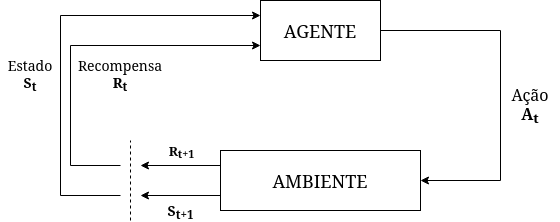
\includegraphics[scale=0.75]{figs/RL-diagram.drawio.png}
    \caption{diagrama da interação do agente com o ambiente. Adaptado de \citeonline{rl-sutton-barto}}
    \label{fig:prefixt}
 \end{figure}

A \textit{política} é o mapeamento do estado percebido do ambiente em ações a serem tomadas naquele estado, é a fórmula que determina qual a decisão correta dadas as observações do ambiente. A política pode ser estocástica, especificando probabilidades para cada ação, algumas maiores que outras.

A recompensa é o número a ser maximizado pelo agente aprendiz, ele indica se o mesmo cumpriu ou está se comportando como deveria. A cada passo, o agente ajusta suas ações com base no sinal de recompensa recebido, se o mesmo é positivo ele deve entender que as ações que tomou foram apropriadas, caso contrário deve buscar mudar seu comportamento a fim de buscar recompensas maiores. Punir em excesso o agente por cometer erros, na intenção de ter um treino mais rigoroso, pode acabar deixando-o sem orientação do que fazer, por outro lado, recompensá-lo demasiadamente pode fazê-lo com que aja inapropriadamente sem se atentar às consequências.

O valor de um estado no ambiente é o tanto de recompensa que o agente espera ganhar no futuro partindo daquele estado. Se o sinal de recompensa indica o que é bom em curto prazo, o valor do estado indica o quanto o agente pode ganhar no longo prazo, talvez \textit{vale} mais a ele ganhar uma recompensa menor se no longo prazo ele receber um montante maior. Recompensas são o objetivo primário, enquanto valores, que são predições de recompensas futuras, são secundários. Se não há recompensas não haverá valores, porém é este último que requer mais atenção de um pesquisador treinando um agente via aprendizado por reforço. Enquanto que recompensas são fáceis de definir, pois basta punir quando algo indesejado ocorrer e premiar caso contrário, maximizar o valor é mais complexo, o agente pode criar o vício de fazer o errado para ganhar recompensas maiores. E é de interesse do aprendizado que o agente tome decisões que leve a maiores valores e não maiores recompensas.

\subsection{Algoritmos de otimização de política}
Nesta seção será abordado mais sobre os diferentes tipos de algoritmos de otimização de política, principalmente o PPO, SAC que estão disponíveis no ML-Agents da Unity 3D.
\chapter{Estado da Arte}\label{cap:estArte}
Neste capítulo será discutido e analisados trabalhos que envolve a criação de agentes inteligentes em ambientes virtuais, a primeira seção será dedicada àqueles que não utilizam o pacote ML-Agents. A outra seção, porém será visto projetos que se utilizam da biblioteca da Unity3D.

\section*{CARLA e outros}
Um projeto muito similar ao que este artigo se propõe a fazer é o \textbf{CARLA}. Car Learning to Act (CARLA) é um ambiente de código aberto de treinamento condução autônoma de veículos terrestres, foi desenvolvido usando a \textbf{Unreal Engine 4}. A simulação inclui clima dinâmico, uso de visão computacional, obstáculos dinâmicos como carros e pedestres além de visual fotorrealista. Quanto ao treinamento utiliza-se de três métodos: um fluxo modular, aprendizado por imitação e aprendizado por reforço, treinaram os agentes em cada método em 4 níveis diferentes de dificuldade, e então postos a testes em climas e uma cidade distinta. O resultado foi surpreendente, com o aprendizado por reforço tendo um desempenho muito inferior aos outros dois métodos (\citeonline{pmlr-v78-dosovitskiy17a}).


\section*{Criação de agentes inteligentes utilizando ML-Agents}\label{sec:primTrab}
O projeto desenvolvido por (\citeonline{s21020492}) também envolve um carro autônomo, apesar de não envolver um ambiente urbano e sim uma pista em formato de 8 (para treino) e outra com começo e fim (para teste). O trabalho analisa o dados da dirigibilidade comparando um humano em um simulador, um agente criado usando aprendizado por imitação e outro agente utilizando \textbf{RL}. 

Outro trabalho foi feito por (\citeonline{mexas2021}), que também se trata de um veículo autônomo, mas desta vez é um veleiro. Neste projeto, o autor faz um estudo comparativo dos algoritmos \textbf{PPO} e \textbf{SAC} para aprendizado por reforço, e os algoritmos \textbf{BC} e \textbf{GAIL} para \textbf{IL}. O ambiente dele leva em conta a ação do vento sobre o veleiro e ao analisar os dados conclui que o primeiro algoritmo de \textbf{RL} é o que apresentou o melhor desempenho.

% PARTE
\part{Metodologia}
\chapter{Ferramentas}\label{cap:ferramentas}

Para criar o projeto foi usado a Unity3D na versão \textbf{2022.3.7f1}. Acerca do \textbf{ML Agents}, há dois pacotes, o primeiro para o editor da Unity3D que adiciona os componentes e classes de \textbf{RL} e \textbf{IL}, esta está na versão \textbf{2.0.1}. O outro pacote seria o pacote Python \textbf{mlagents-learn}, instalado via \textbf{pip}(gerenciador de pacotes do Python), este encontra-se na versão \textbf{0.30.0}. 

Como foi dito, para fazer o agente treinar é necessário criar um ambiente Python que interage com o editor da Unity informação, para isto foi usado Python na versão \textbf{3.9.13}, a principal dependência Python do \textbf{mlagents} é o \textit{framework} \textbf{PyTorch}, neste projeto usa-se a versão \textbf{1.7.1}. As demais dependências Python estão presentes no requirements.txt disponíveis online no repositório oficial deste projeto que se encontra em \href{https://github.com/antunesvitor/SimuladorDeConducao}{https://github.com/antunesvitor/SimuladorDeConducao}

A Unity e o Python estão presentes em para Windows e Linux, ambos os sistemas operacionais foram usados para o desenvolvimento deste projeto, porém grande parte dos testes foram conduzidos no \textbf{Arch Linux} utilizando-se do Kernel \textbf{6.4.10-arch1-1}.

%Inserir aqui a versão do windows

No repositório mencinado acima encontra-se também instruções de instalação tanto no \textbf{Windows} quanto no \textbf{Arch Linux}.

Para a criação do ambiente, foi utilizado dois \textit{assets} da Unity Asset Store, ambos fornecem os modelos 3D necessários para montar o ambiente de treino. O primeiro fornece modelos de carros que servirão como o agente (\citeonline{arcade-free-car-unity-asset}) o outro contém diversos modelos necessários para a construção da cidade como ruas, calçadas, prédios, residências, árvores, postes, etc. (\citeonline{city-package-unity-asset})

% Criar um README.md no repositório com as instruções
\chapter{Modelo proposto}\label{cap:proposta}
Este capítulo abordará o sistema de treinamento proposto, será exposto como funciona todo o ambiente simulado. Dentre os módulos que compõe um veículo autônomo o foco deste projeto será em desenvolver o componente de controle de deslocamento que é responsável por fazer carro percorrer um trajeto. No mundo real as rotas seriam geradas por outro componente, porém isto está além do escopo deste projeto, portanto elas serão definidas pelo autor. Importante ressaltar que o conjunto de rotas deve ser composto por uma variedade de trajetos que exijam uma diversidade de manobras a serem aprendidas pelo agente.

% Esta seção está sujeita a mudanças feitas no ambiente durante o PGCIII. 
\section{Modelo}\label{modelo}
Aqui é descrito sobre o modelo do projeto. Por "modelo" entende-se o conjunto ambiente-agente-recompensas. Cada um deles é detalhado nas subseções abaixo.

\subsection{O ambiente}
A simulação envolve em treinar o veículo para percorrer trajetos em ambiente urbano, a princípio, por uma questão de simplicidade o agente não terá de lidar com declives ou aclives, semáforos, outros veículos ou pedestres. Porém outros elementos estáticos comuns de uma cidade como calçadas, postes, árvores, prédios, etc. Portanto, o foco poderá se manter no estudo de fazer um agente percorrer as rotas. Às bordas do cenário há muros que limitam o alcance do veículo, foi concluído pelo autor que o tamanho atual é suficiente para os treinos iniciais, em estudos futuros pode ser considerado a expansão do cenário. O agente recebe uma punição ao se chocar com a calçada ou com os muros da borda da cidade.

\begin{figure}[h]
   \centering
   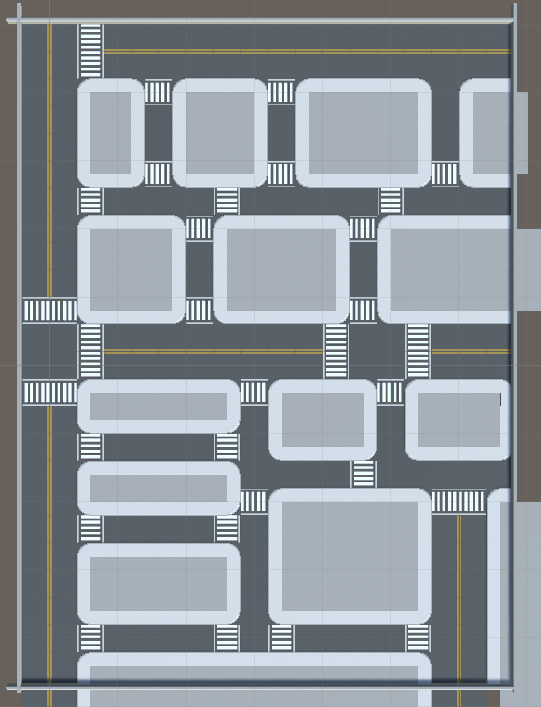
\includegraphics[scale=0.45, angle=90]{figs/Mapa-simulador-visao-superior.png}
    \caption{Visão superior o cenário urbano criado para o treinamento do veículo}
    \label{fig:map-view}
 \end{figure}

As rotas são compostas por: origem, \textit{checkpoints} e destino. O primeiro indica o local de partida do veículo, o último é o objetivo final do agente naquele episódio. Os \textit{checkpoints} são barreiras que indicam o caminho que deve ser percorrido, cada vez que o veículo atravessa uma delas ele ganha uma recompensa, isto é uma forma de indicar a ele que está fazendo o correto. Há 17 percursos predefinidos, cada uma delas possuem características distintas como distância origem-destino, quais e quantas conversões a serem feitas, isto foi moldado visando trazer uma diversidade maior de desafios a serem superados pelo agente. Assim como o tamanho do cenário, novos trajetos podem ser considerados em estudos futuros.

\begin{figure}[h]
   \centering
   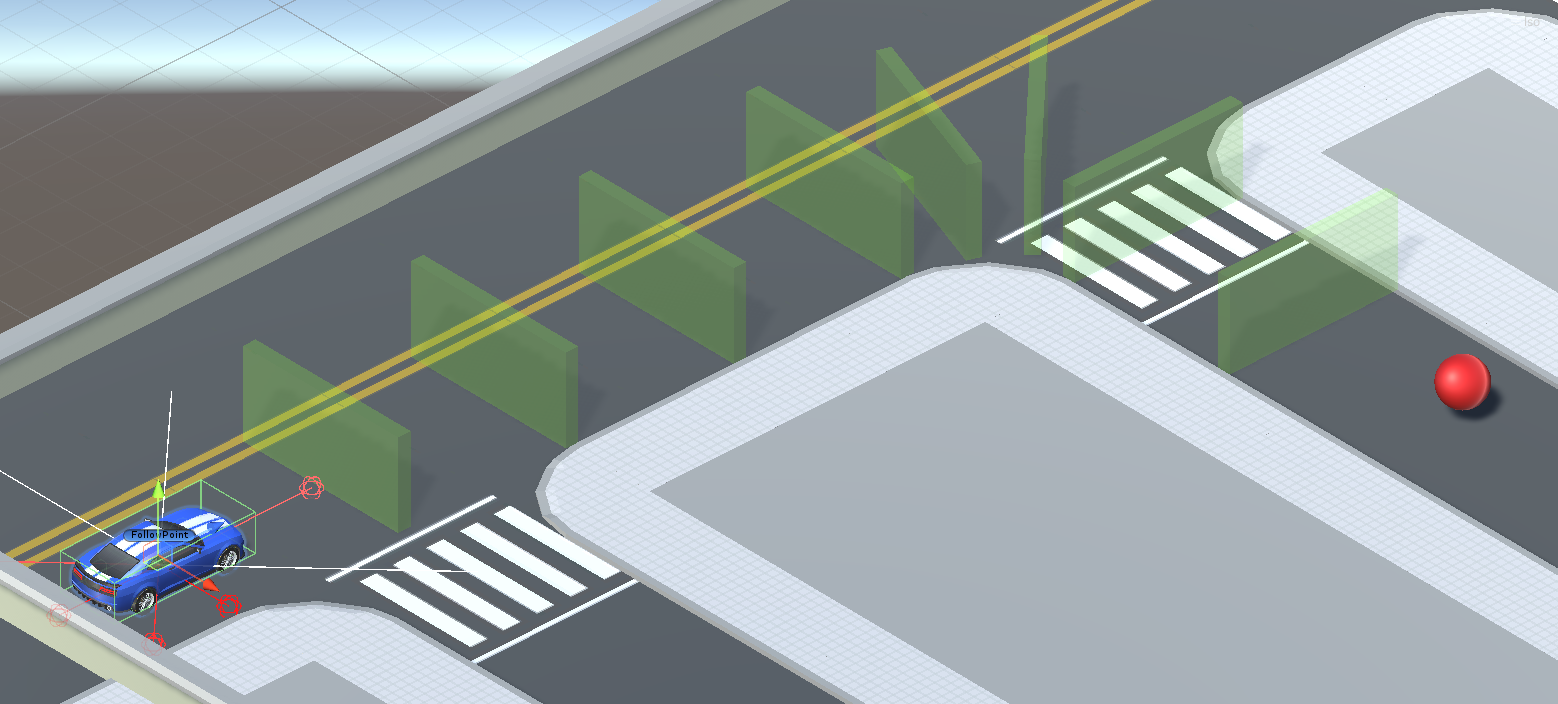
\includegraphics[scale=0.35]{figs/detalhe-rota.png}
    \caption{Rota vista de perspectiva isométrica, o agente posicionado a origem ao canto esquerdo, com os \textit{checkpoints} ao longo do percurso até o destino no canto direito.}
    \label{fig:route-view}
 \end{figure}

 \subsection{O agente}
 Para o aprendizado o veículo possui 8 sensores apontando para todas as direções uniformemente espaçadas, estes sensores são um \textit{component} do pacote \textbf{ML-agents} da Unity3D, são capazes de medir a distância dos objetos próximos ao veículo e também são capazes de distinguir quais são estes objetos. Estes sensores dentro do editor são representados por feixes que partem do centro do veículo, é possível configurar diversos atributos deles como a quantidade, o ângulo máximo de distância do primeiro ao último, o ângulo vertical (que indica se eles apontam para cima ou para baixo) e o tamanho da esfera, que nada mais é que a tolerância de colisão do sensor.

 \begin{figure}[h]
   \centering
   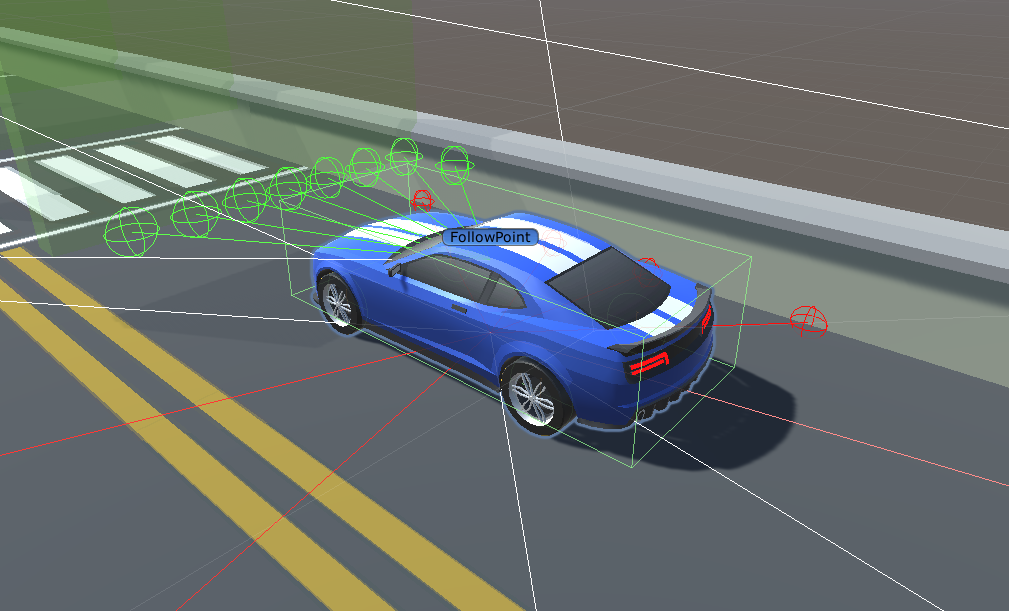
\includegraphics[scale=0.35]{figs/agente-raios-checkpoint.png}
    \caption{Exemplo do agente e seus raios perceptores, é possível ver 6 raios laterais se chocando com as calçadas ao lado, o raio frontal se chocando com o \textit{checkpoint}.}
    \label{fig:casting-rays}
 \end{figure}

 Além dos sensores, foi adicionado a velocidade do veículo a lista de observações do agente. Vale lembrar que o não foi implementado um recurso de imagem em um primeiro momento, ou seja, o veículo só enxerga através dos sensores e tem ciência de sua própria velocidade, ele é "cego" a qualquer outro elemento do ambiente que não esteja se choccando com o sensor.

 Quanto as ações que o agente pode fazer são apenas 3: acelerar, frear e direcionar as rodas a direita e a esquerda. A primeira e a última ação são chamadas ações contínuas, sendo assim um número que indica o nível de aceleração que o carro irá produzir, e no caso da direção da roda o quão direciona elas estão a esquerda ou direita. O ato de frear por outro lado é uma grandeza discreta, o veículo está ou não está freando.

\subsection{As recompensas}
Dado os sensores do agente e o ambiente montado podemos definir as recompensas/punições das seguintes ocorrências: chegar ao destino ($R_d = 1$, sempre), atingir um \textit{checkpoint} ($R_c$), colidir com a/subir na calçada ($P_c$), colidir com a parede($P_p$), não chegar no destino a tempo($P_t$). Além disso temos os seguintes cenários possíveis: o agente chega ao destino, o agente não chegar a tempo, o agente tombar o veículo. As recompensas estão no intervalo $[-1,1]$ e serão aplicadas da seguinte forma em cada cenário:

\begin{itemize}
   \item Chega ao destino: $R_T = R_d - P_c - P_p$
   \item Não chega a tempo: $R_T = R_c - P_c - P_p$
   \item Tomba o carro: $R_T = -1$
\end{itemize}

\section{Os algoritmos e hiper-parâmetros}\label{algoritmos}
Para executar o treino é necessário especificar para o \textbf{ml-agents} o algoritmo e suas configurações, para isso existe um arquivo \textbf{.yaml} que é responsável por isso. Abaixo, um exemplo seguido da explicação de cada parâmetro:

\begin{lstlisting}
behaviors:
   MoveToTarget:
      trainer_type: ppo
      max_steps: 9600000
      time_horizon: 64
      summary_freq: 60000
      keep_checkpoints: 16     
      checkpoint_interval: 600000
      hyperparameters:
         learning_rate: 1.0e-5
         batch_size: 1024
         buffer_size: 10240
         beta: 5.0e-2
         epsilon: 0.1
         lambd: 0.99
         num_epoch: 8
         learning_rate_schedule: linear
         beta_schedule: linear
         epsilon_schedule: linear
      network_settings:
         normalize: false
         hidden_units: 64
         num_layers: 2
      reward_signals:
         extrinsic:
            gamma: 0.99
            strength: 1.0
\end{lstlisting}

O arquivo começa com o \textbf{behaviors} que é uma lista de configurações dos comportamentos do agente, neste projeto haverá apenas um que é chamado \textbf{MoveToTarget}. Abaixo segue uma lista dos hiper-parâmetros mais relevantes, o texto aqui é em grande parte traduzido da documentação oficial do \textbf{ml-agents} (\citeonline{juliani2020}) com algumas remoções de informações não relevantes pra este projeto e com alguns adendos do autor caso necessário.

\begin{description}
   \item [trainer\_type:] O algoritmo que será usado, neste projeto serão PPO ou SAC
   \item [max\_steps:] O número máximo de passos(observações coletadas e ações tomadas pelo agente) tomados  no ambiente. No simulador a tarefa sempre será episódica, o tamanho do episódio pode variar nos ajustes, mas cada um possui em torno de 1200 \textit{steps}.
   \item [time\_horizon:] O número de \textit{steps} anteriores a ser coletado por agente para adicionar ao \textit{buffer} de experiência. Quando este limite é alcançado antes do fim de um episódio, um valor estimado é usado para prever a expectativa geral de recompensa a partir do estado atual do agente. Por isso, esse parâmetro varia entre menos enviesado mas com alta variância estimada (longo prazo) e mais enviesado mas com estimativa de menor variância (curto prazo). Em casos onde há frequente sinais de recompensas ou em episódios muito longos, um número menor pode ser mais ideal.
   \item [hyperparameters->learning\_rate:] Taxa inicial do salto a cada atualização do gradiente descendente. Este número geralmente deve diminuir com se o treino está instável e a recompensa com aumenta consistentemente.
   \item [hyperparameters->batch\_size:] O número de experiências coletadas para cada atualização do gradiente descendente. Em caso de usar ações contínuas ele deve estar na casa do milhares, caso contrário na casa das dezenas deve bastar.
   \item [hyperparameters->batch\_size:] Número de experiências a ser coletada antes de atualizar o modelo da política. Tipicamente, um buffer size maior corresponde a um treino mais estável. No caso do SAC este número deve ser milhares de vezes maior que um episódio típico, pois o algoritmo deve aprender de experiências velhas quanto mais novas.
   \item [hyperparameters->beta:] (somente PPO) força da regularização da entropia, que faz com que a política seja "mais aleatória". Isto garente que o agente explore apropriadamente o espaço da ação durante o treino. Aumenta-lo faz com que o agente tome mais ações aleatória. Isto deve ser ajustado de modo que o a entropia (medido pelo tensorboard) lentamente decresça conforme aumenta a recompensa. Se a entropia cair muito rápido aumente o \textbf{beta}, caso demore demais diminua-o.
   \item [hyperparameters->epsilon:] (somente PPO) Influencia no quão rapidamente a política pode evoluir durante o treino. Corresponde ao limite da divergência entre as velhas e novas políticas durante a atualização do gradiente descendente. Um valor menor leva a atualizações mais estáveis, mas deixa o processo de aprendizagem mais lento.
   \item [hyperparameters->lambd:] (somente PPO) parâmetro de regularização (lambda) usado quando calculado o estimador de valor generalizado (GAE (\citeonline{1506.02438})). Isto pode ser entendido em o quanto o agente depende no seu atual valor estimado quando atualizando o valor estimado. Valores baixos corresponde a apoiar-se mais no valor atual (alto viés/\textit{bias}) e valores elevados corresponde a confiar mais nas recompensas recebidas pelo ambiente (que pode causar alta variância). (geralmente varia de 0,9 a 0,99)
   \item [hyperparameters->num\_epoch:] (somente PPO) O número de passagens a fazer pelo buffer\_size quando otimizando gradiente descendente. Este deve crescer semelhante ao batch\_size. Diminui-lo tende a ter atualizações mais estáveis, aumentá-lo tem-se um treino mais lento. (geralmente varia entre 3 a 10)
   \item [hyperparameters->learning\_rate\_schedule:] Determina se o valor do learning\_rate muda durante o treino, os valores podem ser \textit{linear} ou \textit{constant}. Sendo o primeiro ele irá decair linearmente até zero quanto executar o \textit{max\_steps}. O segundo mantém o valor constante. É recomendado adotar \textit{linear} para PPO e o outro quando usar SAC.
   \item [hyperparameters->beta\_schedule:] (somente PPO) Similarmente ao acima mas para o \textbf{beta}. 
   \item [hyperparameters->epsilon\_schedule:] (somente PPO) Similarmente ao acima mas para o \textbf{epsilon}. 
   \item [hyperparameters->buffer\_init\_steps:] (somente SAC) Número de experiências a coletar no buffer antes de atualizar o modelo da política. Inicialmente o buffer é preenchido com ações aleatórias,o que é muito útil para exploração. Este número deve ser na casa de dezenas de vezes maior que um típico episódio.
   \item [hyperparameters->init\_entcoef:] (somente SAC) Corresponde a entropia inicial definida no começo do treino e é o quanto o agente deve explorar inicialmente. No SAC, o agente é incentivado a tomar decisões aleatorias a fim de explorar melhor o ambiente. O coeficiente de entropia é ajustado automaticamente para um valor alvo predefinido então o \textit{init\_entcoef} é apenas o valor inicial. Quanto maior o valor maior a exploração inicial. Para ações contínuas o típico valor está no invervalo 0,5-1,0, discreto em 0,05-0,5.
   \item [network\_settings->hidden\_units:] O número de nós em cada camada intermediária da rede neural totalmente conectada (valores típicos giram em torno de 32 a 512).
   \item [network\_settings->num\_layers:] O número de camadas intermediárias na rede neural (tipicamente tem valor de 1 a 3).
   \item [network\_settings->normalize:] Se normalização deve ser aplicada no vetor de observação. Esta normalização pode melhorar o treino em caso de tarefas que lidam com controles contínuos complexos, mas pode atrapalhar caso contrário.
\end{description}

\section{Metodologia}
A tarefa a ser resolvida pelo agente é episódica, onde em cada episódio ele terá que chegar ao destino seguindo o trajeto definido pelos checkpoints. O episódio só acaba se ele atingir o destino ou se tombar o veículo. Durante o treino o agente receberá um trajeto aleatório em cada episódio e durante o teste o agente terá que percorrer três vezes todos trajetos na ordem de cada um deles no projeto da Unity. No final terá o desempenho dele no teste será medido tanto quantitativamente quanto dissertativamente. Quantitativamente pois será mostrado o desempenho em cada rota, quantidade (de 0 a 3) de que conseguiu chegar ao destino em cada um deles e quantas colisões foram registradas no total. Dissertativamente será a análise textual com opnião do autor sobre a condução do veículo e focará em observar características mais subjetivas (por exemplo se o agente conduz o carro com muitas revoluções ou se acelera e freia muito bruscamente, entre outras). 

Como foi dito na seção \nameref{sec:objetivos}, o propósito deste projeto é estudar a criação e desenvolvimento de um ambiente simulado para o treino de veículo autônomos, logo o mesmo está sujeito a mudanças e melhorias para tornar a simulação o mais próximo da realidade possível. O versionamento do modelo será definido aqui, suas mudanças mais relevantes serão detalhadas e justificadas, mudanças estas que incluem alterações de recompensas, observações do agente, hiper-parâmetros dos algoritmos PPO e SAC. Vale ressaltar que as mudanças seguem na ordem da maior pra menor: alteração do agente ou ambiente, reorganização das recompensas, ajustes nos hiper-parâmetros. Não são todos os ajustes que serão expostos aqui, especialmente ao dos hiper-parâmetros, se um alteração não levar a um resultado diferente antes de outro reajuste então pode ser considerado insignificante.

\subsection{Treinamento e teste}
Tendo o \nameref{modelo} e \nameref{algoritmos} detalhados acima é preciso explicar o treinamento e teste. O treinamento é executado via linha de comando, é necessário ativar o ambiente Python, gerar um executável do simulador pelo editor da unity e ter um arquivo de configuração do algoritmo. Tendo estes três itens é possível executar o comando do ml-agents e por o agente em treino. Após o treino finalizar é gerado um arquivo \textbf{.onnx} que é política final do agente, a rede neural com os coeficientes gerados pelo algoritmo após o treino, o seu "cérebro". Finalmente podemos por o agente em teste, de volta ao editor da Unity3D, basta carregar o cérebro no agente e executar o teste, o veículo agora se mexe sozinho sem input do usuário, e o mesmo deve estar agindo de acordo com os resultados do treino, seja ele um sucesso ou não.

Nos testes o agente deverá percorrer os mesmos trajetos, agora eles não serão aleatórios, ele percorrerá cada um três vezes. Como na lista de observações não inclui qualquer informação sobre qual trajeto ele está percorrendo no momento, o autor não viu necessidade de separar trajetos de treino e de teste, embora essa possibilidade posta em estudos futuros.

\subsubsection*{Estatísticas de treino}
Quando o treino é finalizado é armazenado diversas estatísticas que são exibidas pelo \textbf{tensorboard}. Nelas é possível ter uma visualização do desempenho do agente durante o treino e sua curva de aprendizado. As que serão analisadas e discutidas na próxima parte estão descritas na lista abaixo. Assimi como a listagem dos hiper-parâmetros essas definições são traduções diretas da documentação do ML-agents (\citeonline{juliani2020}).

\begin{description}
   \item [Cumulative Reward:] A mediana da recompensa acumulada no episódio do agente. Deve aumentar ao longo de um treino bem sucedido (Esta estatística possui dois gráficos, um de linha e outro histrograma)
   \item [Episode Length:] A duração mediana dos episódios (No caso deste projeto a duração deve diminuir ao longo do tempo, pois significa que o agente está realizando a tarefa mais eficientemente).
   \item [Entropy:] a entropia da política, isto é, o quão aleatório as decisões do modelo são. Deve decair durante um treino bem sucedido. Se decair muito rapidamente deve-se aumentar o valor do hiperparâmetro \textbf{beta}.
   \item [Extrinsic value estimate:] É a mediana do valor de todos os estados visitados pelo agente. Deve aumentar ao longo de um treinamento bem sucedido.
\end{description}

Os demais gráficos são o \textbf{beta}, \textbf{epsilon} e \textbf{learning\_rate} eles são basicamente o valor destes hiper-parâmetros ao longo do treino, dependendo se os \textit{schedules} deles forem constante ou linear, é esperado uma linha constante no primeiro caso ou uma queda do valor deles até zero caso linear.

\subsection{Estudo e análise}
Será estudado um modelo por vez, a descrição do modelo acima está sujeita a mudanças, a descrição acima é a primeira versão e todas as alterações que foram necessárias serão expostas, detalhadas e justificadas na seção de Resultados e Discussão. Cada modelo será treinado e testado com ambos os algoritmos, os hiperparametros não serão iguais para ambos pois a ideia é extrair o melhor resultado de ambos os cenários. A análise pretende responder as seguintes perguntas:

\begin{itemize}
   \item Algum algoritmo convergiu relativamente rápido? Se sim qual deles?
   \item Algum algoritmo obteve uma média de recompensa satisfatória? Qual obteve a melhor?
   \item Caso positivo pra pergunta acima, algum desempenho satisfatoriamente nos testes? Qual foi o melhor?
\end{itemize}

Se as respostas para as perguntas acima forem negativas, o cáculo de recompesas será alterado, caso persista os observadores do agente será alterado. Até que se obtenha um agente eficiente.

%%%%%
% Comentar sobre: 
% Como será o teste:
%     considerar criar uma rotina de teste 
%%%%
 

% PARTE
\part{Parte Final}
\chapter{Resultados e Discussão}\label{cap:resultados}

% \section{Desafio em trajeto especifíco fácil}

% O primeiro e único treino foi executado como agente percorrendo somente um percurso em linha reta, conforme a imagem abaixo.

% \begin{figure}[h]
%     \centering
%     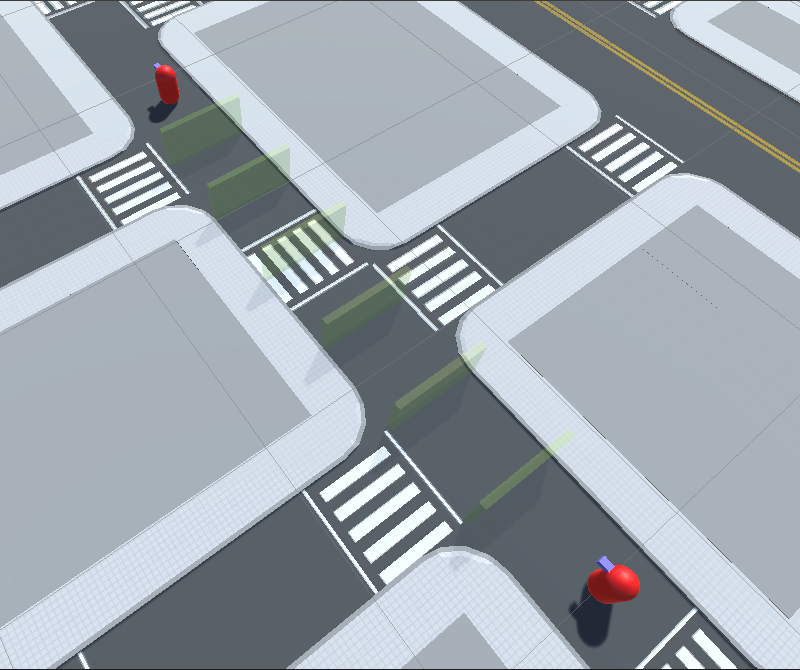
\includegraphics[scale=0.25]{figs/rotas/path_14.png}
%      \caption{O percurso executado no primeiro treino. A cápsula vermelha no canto inferior direito indica a posição inicial do veículo e a na parte superior esquerdo indica o destino.}
%      \label{fig:rota-1}
% \end{figure}
 
% \begin{figure}[h]
%     \centering
%     \includegraphics[scale=0.35]{figs/treinos/treino-1/política.png}
%      \caption{Estatísticas referentes a política. O primeiro gráfico é a entropia, decaindo como é esperado. O terceiro gráfico é o Extrinsic Value estimate, sobe e estabiliza, conforme esperado}
%      \label{fig:treino-1-politica}
% \end{figure}

% \begin{figure}[h]
%     \centering
%     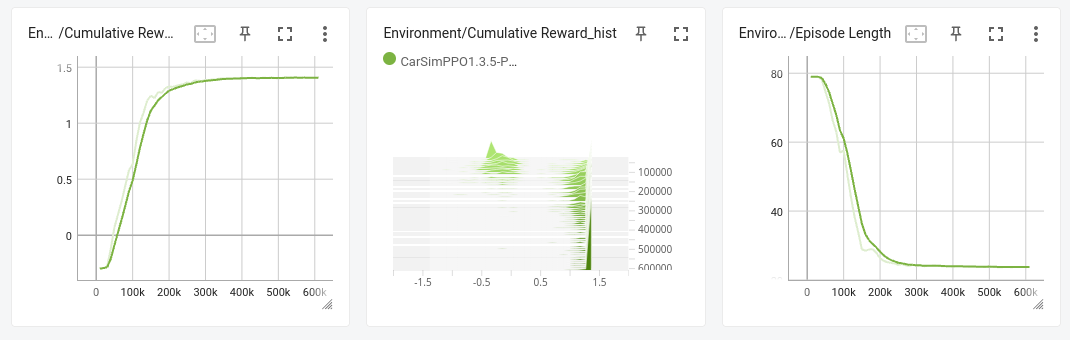
\includegraphics[scale=0.35]{figs/treinos/treino-1/ambiente.png}
%      \caption{Estatísticas do ambiente. O primeiro gráfico é o acumulado de recompensa, o segundo é um histograma das distribuições de recompens. O terceiro é a duração do episódio.}
%      \label{fig:treino-1-ambiente}
% \end{figure}

% \subsection*{Análise}
% O treino foi bem sucedido, o agente soube conduzir bem o veículo. Vendo o gráfico 1 da figura 9, pode-se notar o crescimento exponencial da recompensa e então sua estabilização quando atinge o máximo da recompensa que é possível receber. Também percebe-se que na mesma velocidade mas desta vez em sentido descendente a duração média do episódio, rapidamente cai pois o agente já dominou o trajeto. Isso é o suficiente para este trajeto, podemos treinar o agente em um novo desafio especifíco mas com um trajeto mais complexo.


\section{Desafio em trajeto específico dificuldade fácil}
Aqui o treino foi feito em dois trajetos (identificados por Path(8) e Path(0) no projeto), ambos exigem que o agente faça uma conversão do veículo.

\begin{figure}[h]
    \centering
    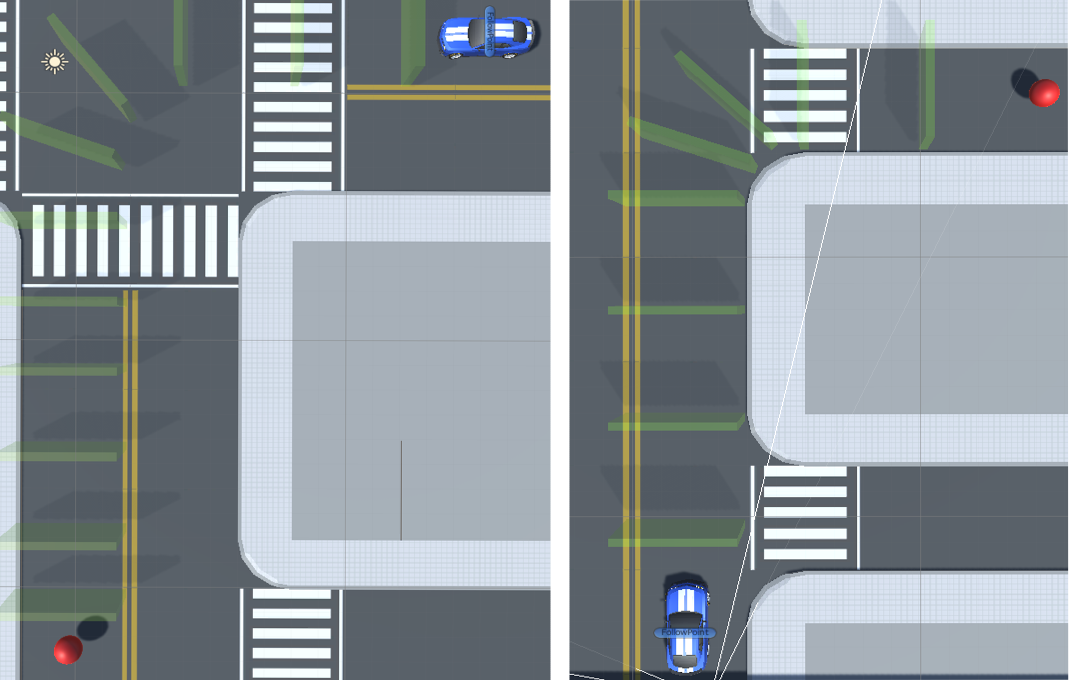
\includegraphics{figs/treinos/desafio-mediano/paths_0-8.png}
    \caption{Trajetos deste desafio, à esquerda o Path(0) e à direita o Path(8).}
\end{figure}

\begin{figure}[h]
    \centering
    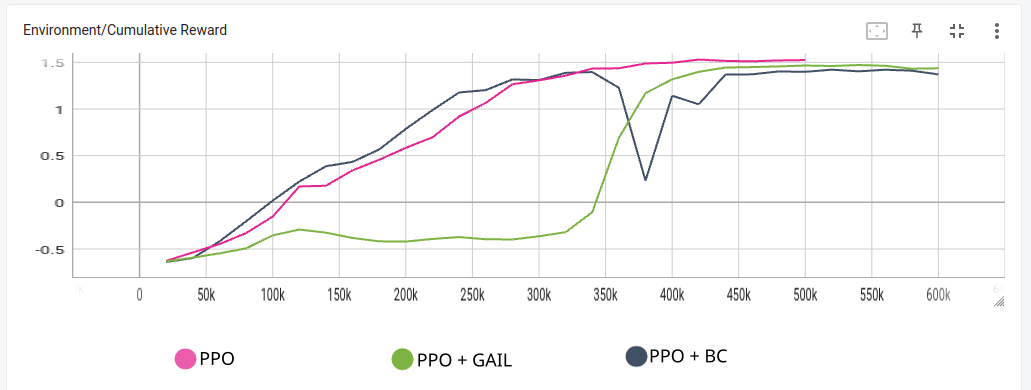
\includegraphics[scale=0.42]{figs/treinos/desafio-mediano/path0/recompensa-ppo-bc-gail-path0.png}
    \caption{Recompensa cumulativa mediana por steps durante o treino do agente no Path(0).}
\end{figure}

\begin{figure}[h]
    \centering
    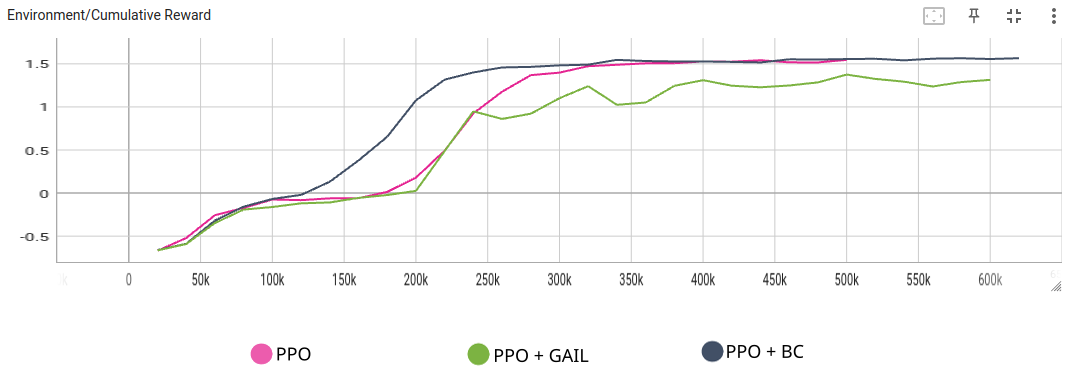
\includegraphics[scale=0.42]{figs/treinos/desafio-mediano/path8/recompensa-ppo-bc-gail-path8.png}
    \caption{Recompensa cumulativa mediana por steps durante o treino do agente no Path(8).}
\end{figure}

O treinamento não encontrou problemas para convergir neste desafio em qualquer dos três algoritmos. PPO foi o que obteve a melhor mediana final no \textit{Path(0)} mesmo dispondo de menos \textit{steps} para treinar. Embora tenham convergido, GAIL e BC se mostrando instáveis, o primeiro demorou muito para mostrar alguma melhora no agente enquanto o último apresentou uma anomalia no Path(0) após 350 mil \textit{steps} voltando a se estabilizar após 450 mil passos. Quanto ao \textit{Path(8)}, o treino utilizando-se de BC convergiu mais rápido e também obteve a maior mediana, enquanto que GAIL foi o mais instável, não convergindo.

\begin{table}[htpb]
    \centering
    \caption{Consolidado de resultados por rota e algoritmo, contém a mediana final da recompensa no treino, o desempenho testes é quantas rotas completou de quantas tentativas e média de recompensas nos testes.}
    \label{resultado-tabela-desafio-1}
    \begin{tabular}{|l|c|c|c|c|c|c|r|}
         \hline
         \small{Rota} & \small{Algoritmo}   & \small{Mediana final rec. treino}  & \small{Desempenho testes}    & \small{Média rec. testes} \\ \hline
            Path(0)   &      PPO            &   1.524                            &    10/10                     &      1                    \\ \hline
            Path(0)   &      GAIL           &   1.436                            &    10/10                     &      1                    \\ \hline
            Path(0)   &      BC             &   1.371                            &    10/10                     &      1                    \\ \hline
            Path(8)   &      PPO            &   1.546                            &    10/10                     &      1                    \\ \hline
            Path(8)   &      GAIL           &   1.314                            &    6/10                      &      0.585                \\ \hline
            Path(8)   &      BC             &   1.565                            &    10/10                     &      1                    \\ \hline
    \end{tabular}
\end{table}


Nos testes, com exceção do algoritmo GAIL no \textit{Path(8)}, foram quase sem qualquer falha. O  cérebro treinado com o algoritmo BC subiu na calçada uma vez em cada teste, mas a punição por uma ocorrência não é suficiente pra afetar a média.

\section{Desafio em trajeto específico difícil}
Para este desafio foi testado em três rotas diferentes: \textit{Path(3), Path(5) e Path(6)}. A primeira é a mais complexa contém três curvas alternadas, enquanto \textit{Path(5)} requer que o carro faça duas conversões a direita e o último trajeto possui duas curvas alternadas. 

Neste desafio ficou claro que o agente teve dificuldade em convergir nos algoritmos BC e GAIL no Path(3), com BC tendo um crescimento constante seguido de uma queda gradual de desempenho até atingir o patamar mais baixodos três, enquanto GAIL ficou estagnado em um mínimo local assim como fez no Path(5). No Path(6) todos convergiram, com PPO com uma mediana consideravelmente maior.

\begin{figure}[h]
    \centering
    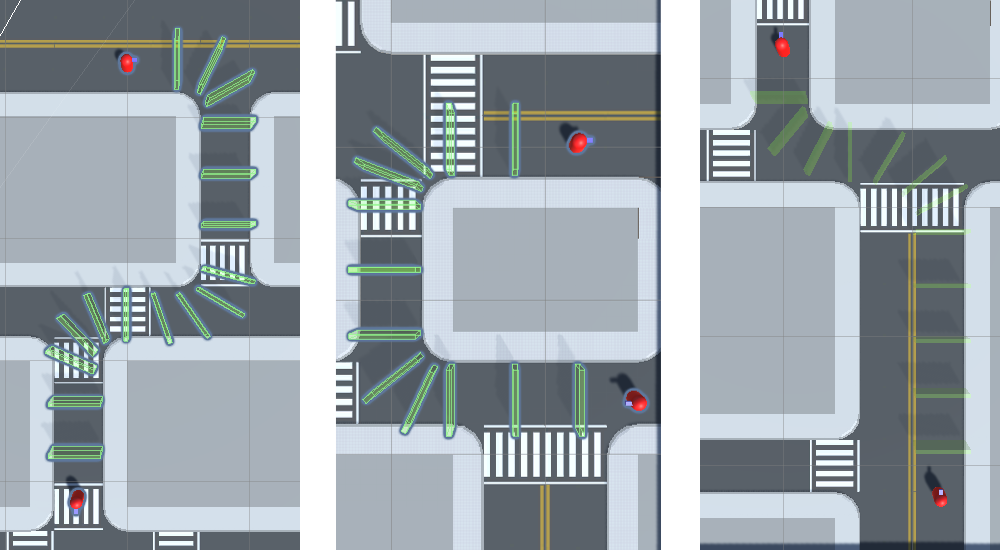
\includegraphics{figs/treinos/desafio-dificil/rotas.png}
    \caption{As três rotas difíceis envolve mais de uma curva, a esquerda o path(3) que possui três curvas sendo o mais complexo dos trajetos. Os outros dois são o path(5) e path(6) que possuem 2 curvas cada.}
\end{figure}

\begin{figure}[h]
    \centering
    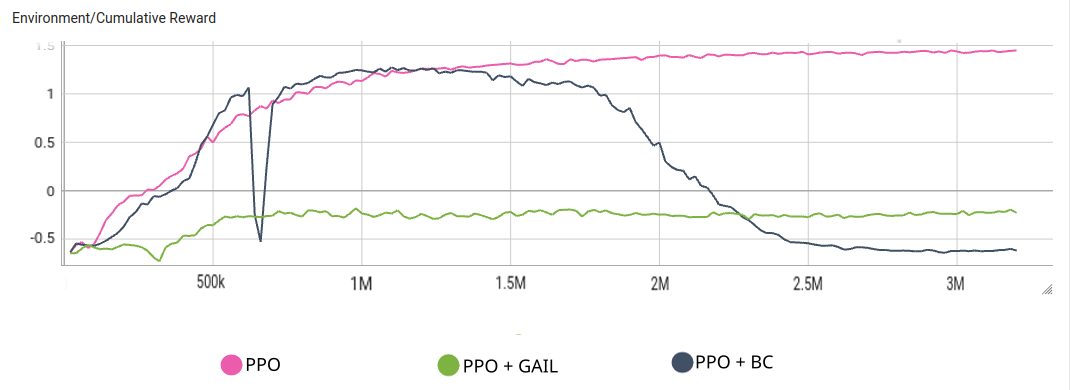
\includegraphics[scale=0.35]{figs/treinos/desafio-dificil/path-3_recompensas-algos.png}
    \caption{Recompensa cumulativa mediana por steps durante o treino do agente no Path(3).}
\end{figure}

\begin{figure}[h]
    \centering
    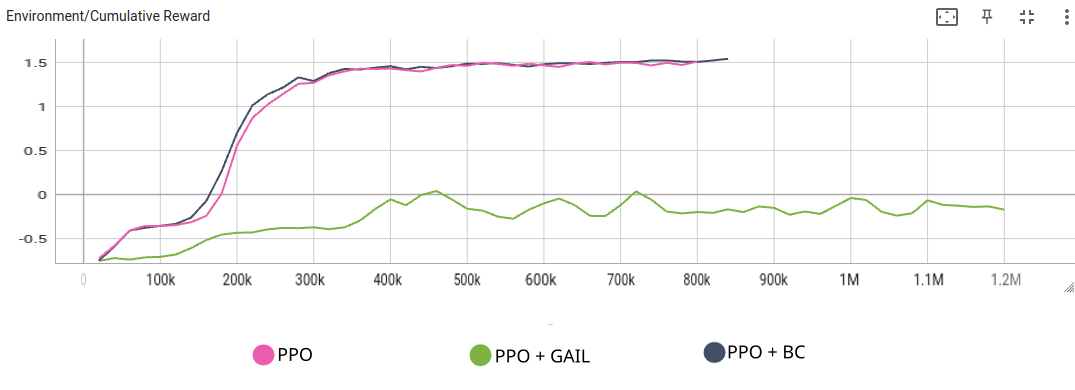
\includegraphics[scale=0.35]{figs/treinos/desafio-dificil/path-5_recompensas-algos.png}
    \caption{Recompensa cumulativa mediana por steps durante o treino do agente no Path(5).}
\end{figure}

\begin{figure}[h]
    \centering
    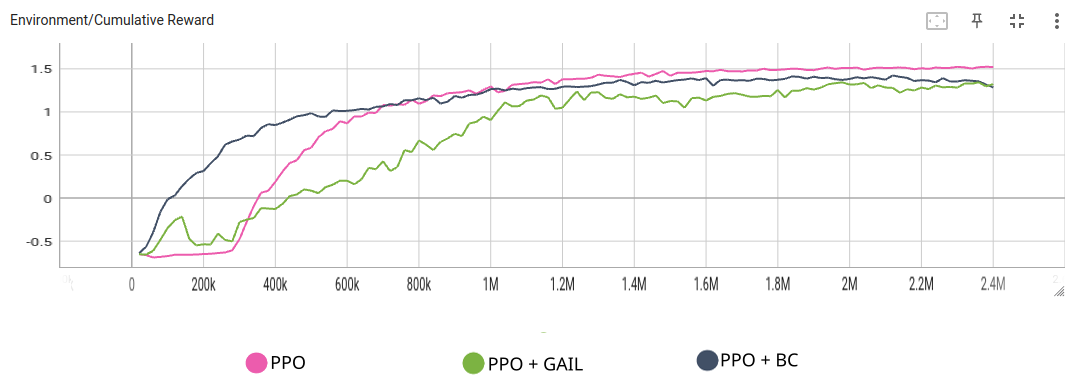
\includegraphics[scale=0.35]{figs/treinos/desafio-dificil/path-6_recompensas-algos.png}
    \caption{Recompensa cumulativa mediana por steps durante o treino do agente no Path(6).}
\end{figure}

\begin{table}[htpb]
    \centering
    \caption{Consolidado de resultados por rota e algoritmo do segundo desafio.}
    \label{resultado-tabela-desafio-2}
    \begin{tabular}{|l|c|c|c|c|c|c|r|}
         \hline
         \small{Rota} & \small{Algoritmo}   & \small{Mediana final rec. treino}  & \small{Desempenho testes}    & \small{Média rec. testes} \\ \hline
            Path(3)   &      PPO            &   1,449                            &    10/10                     &      0,97                 \\ \hline
            Path(3)   &      GAIL           &   -0,229                           &    0/10                      &      -0,261               \\ \hline
            Path(3)   &      BC             &   -0,618                           &    0/10                      &      -0.693               \\ \hline
            Path(5)   &      PPO            &   1,509                            &    10/10                     &      0,98                 \\ \hline
            Path(5)   &      GAIL           &   -0,171                           &    0/10                      &      -0,252               \\ \hline
            Path(5)   &      BC             &   1,505                            &    10/10                     &      1                    \\ \hline
            Path(6)   &      PPO            &   1,522                            &    10/10                     &      0,993                \\ \hline
            Path(6)   &      GAIL           &   1,323                            &    10/10                     &      0,99                 \\ \hline
            Path(6)   &      BC             &   1,284                            &    5/10                      &      0,42                 \\ \hline
    \end{tabular}
\end{table}

Todos desempenharam de acordo com o treino durante os testes com exceção do BC no Path(6) concluiu apenas metade das rotas. Durante o teste do Path(6) foi observado uma diferença interessante entre o agente treinado com PPO que usa apenas RL e o GAIL que utiliza-se de IL: o primeiro tendia a abusar de uma falha de detecção de colisão do veículo com a calçada poupando assim um pouco de tempo (e de punição por step) em vez de seguir na via. Isso ocorre porque da forma que o agente passa sobre a calçada o modelo raramente detecta uma colisão ali, com o agente treinado em GAIL isto não ocorre, já que o mesmo tenta imitar o comportamento na demonstração feita por um humano que seguiu na via normalmente.

\section{Desafio em todos os trajetos}
Neste desafio houve uma discrepância muito grande entre GAIL e os outros dois, este último não teve um treino estável mesmo após diversos ajustes nos hiperparâmetros e isto refletiu nos testes onde obteve uma recompensa média negativa. Nas tabelas \ref{resultado-tabela-geral-ppo} e \ref{resultado-tabela-geral-bc} pode-se ver que ambos tiveram mais dificuldades no \textit{Path(10)} que possui duas curvas pra esquerda. Interessante ressaltar que BC nestes testes conseguiu concluir o Path(3) em todas as tentativas em contraste com o desafio anterior onde falhou em todas as dez tentativas, o que nos leva a crer que treinar em outros trajetos ajude o agente a cumprir um trajeto específico em vez de treinar somente em um único trajeto, pelo menos utilizando-se de Aprendizado por Imitação.

\begin{figure}[h]
    \centering
    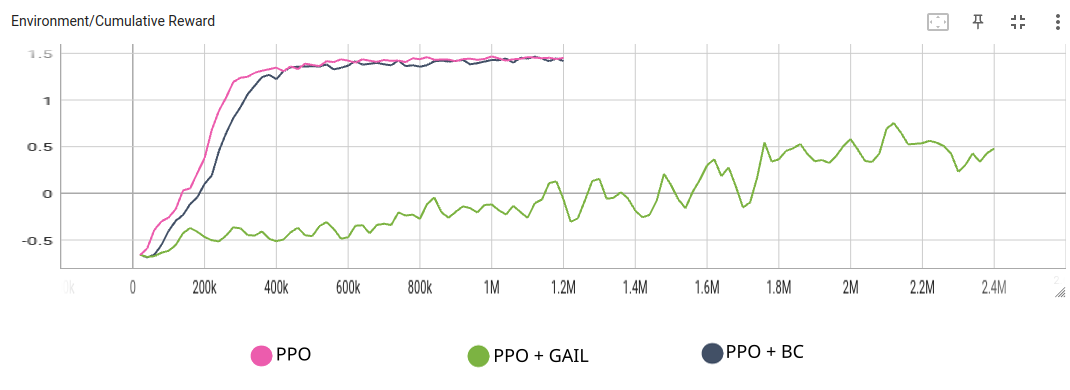
\includegraphics[scale=0.35]{figs/treinos/desafio-geral/recompensa-ppo-gail-bc.png}
    \caption{Recompensa cumulativa mediana por steps durante o treino do agente em todos os trajetos.}
\end{figure}

\begin{table}[htpb]
    \centering
    \caption{Detalhamento do desempenho no teste do desafio geral de PPO, inclui todas tentativas e suas recompensas e a recompensa média por rota.}
    \label{resultado-tabela-geral-ppo}
    \begin{tabular}{|l|c|c|c|c|c|c|r|}
         \hline
         \multirow{2}{*}{Rota} & \multicolumn{2}{c|}{Tentativa 1}  & \multicolumn{2}{c|}{Tentativa 2} & \multicolumn{2}{c|}{Tentativa 3} & \multirow{2}{*}{Rec. média} \\ \cline{2-7}
                               & \small{Concluiu?}  & \small{Rec.} & \small{Concluiu?} &\small{Rec.} & \small{Concluiu?} &\small{Rec.} &                               \\ \hline
            Path(0)   &      sim        &   1             &    sim          &      1        &    sim          &      1        &      1                 \\ \hline
            Path(1)   &      sim        &   1             &    sim          &      1        &    sim          &      1        &      1                 \\ \hline
            Path(2)   &      sim        &   1             &    sim          &      1        &    sim          &      1        &      1                 \\ \hline
            Path(3)   &      não        &   -0,18         &    sim          &      0,85     &    sim          &      1        &      0,56              \\ \hline
            Path(4)   &      sim        &   1             &    sim          &      1        &    sim          &      1        &      1                 \\ \hline
            Path(5)   &      sim        &   1             &    sim          &      0,8      &    sim          &      1        &      0,93              \\ \hline
            Path(6)   &      sim        &   1             &    não          &      -0,31    &    sim          &      1        &      0,56              \\ \hline
            Path(7)   &      sim        &   0,85          &    sim          &      1        &    sim          &      0,9      &      0,91              \\ \hline
            Path(8)   &      sim        &   1             &    sim          &      0,9      &    sim          &      1        &      0,96              \\ \hline
            Path(9)   &      sim        &   1             &    sim          &      0,95     &    sim          &      1        &      0,98              \\ \hline
            Path(10)  &      não        &   0,12          &    não          &      0,02     &    sim          &      1        &      0,38              \\ \hline
            Path(11)  &      sim        &   1             &    sim          &      1        &    sim          &      1        &      1                 \\ \hline
            Path(12)  &      sim        &   1             &    sim          &      1        &    sim          &      1        &      1                 \\ \hline
            Path(13)  &      sim        &   1             &    sim          &      1        &    sim          &      1        &      1                 \\ \hline
            Path(14)  &      sim        &   1             &    sim          &      1        &    sim          &      1        &      1                 \\ \hline
            Path(15)  &      sim        &   1             &    sim          &      1        &    sim          &      1        &      1                 \\ \hline
            Path(16)  &      sim        &   1             &    sim          &      1        &    sim          &      1        &      1                 \\ \hline
    \end{tabular}
\end{table}

\begin{table}[htpb]
    \centering
    \caption{Detalhamento do desempenho no teste do desafio geral de GAIL.}
    \label{resultado-tabela-geral-gail}
    \begin{tabular}{|l|c|c|c|c|c|c|r|}
         \hline
         \multirow{2}{*}{Rota} & \multicolumn{2}{c|}{Tentativa 1}  & \multicolumn{2}{c|}{Tentativa 2} & \multicolumn{2}{c|}{Tentativa 3} & \multirow{2}{*}{Rec. média} \\ \cline{2-7}
                               & \small{Concluiu?}  & \small{Rec.} & \small{Concluiu?} &\small{Rec.} & \small{Concluiu?} &\small{Rec.} &                               \\ \hline
            Path(0)            &      sim          &   1          &    não            &      -0,677 &    sim            &      -0,402 &      -0,026                    \\ \hline
            Path(1)            &      não          &   0,231      &    não            &      -0,01  &    não            &      -0,253 &      -0,011                    \\ \hline
            Path(2)            &      não          &   -0,375     &    não            &      -0,153 &    não            &      -0,551 &      -0,36                     \\ \hline
            Path(3)            &      não          &   -0.412     &    não            &      0,002  &    não            &      -0,588 &      -0,333                    \\ \hline
            Path(4)            &      não          &   -0,086     &    sim            &      1      &    não            &      -0,504 &      0,137                     \\ \hline
            Path(5)            &      não          &   -0,278     &    não            &      0,132  &    não            &      -0,515 &      -0,22                     \\ \hline
            Path(6)            &      sim          &   1          &    sim            &      1      &    não            &      0,201  &      0,734                     \\ \hline
            Path(7)            &      não          &   -0,297     &    não            &      -0,22  &    não            &      -0,636 &      -0,384                    \\ \hline
            Path(8)            &      não          &   0,087      &    não            &      -0,087 &    não            &      0,215  &      0,072                     \\ \hline
            Path(9)            &      não          &   -0,084     &    não            &      0,204  &    não            &      -0,104 &      0,006                     \\ \hline
            Path(10)           &      não          &   -0,44      &    não            &      -0,677 &    não            &      -0,586 &      -0,566                    \\ \hline
            Path(11)           &      não          &   0,063      &    não            &      -0,182 &    sim            &      1      &      0,293                     \\ \hline
            Path(12)           &      não          &   0,074      &    não            &      -0,44  &    não            &      -0,655 &      -0,292                    \\ \hline
            Path(13)           &      nào          &   0,191      &    não            &      -0,686 &    não            &      -0,668 &      -0,718                    \\ \hline
            Path(14)           &      não          &   0,098      &    não            &      -0,644 &    não            &      -0,553 &      -0,366                    \\ \hline
            Path(15)           &      não          &   -0,579     &    não            &      -0,397 &    não            &      -0,47  &      -0,604                    \\ \hline
            Path(16)           &      sim          &   1          &    não            &      -0,665 &    não            &      -0,653 &      -0,106                    \\ \hline
    \end{tabular}
\end{table}

\begin{table}[htpb]
    \centering
    \caption{Detalhamento do desempenho no teste do desafio geral de BC.}
    \label{resultado-tabela-geral-bc}
    \begin{tabular}{|l|c|c|c|c|c|c|r|}
         \hline
         \multirow{2}{*}{Rota} & \multicolumn{2}{c|}{Tentativa 1}  & \multicolumn{2}{c|}{Tentativa 2} & \multicolumn{2}{c|}{Tentativa 3} & \multirow{2}{*}{Rec. média} \\ \cline{2-7}
                               & \small{Concluiu?}  & \small{Rec.} & \small{Concluiu?} &\small{Rec.} & \small{Concluiu?} &\small{Rec.} &                               \\ \hline
            Path(0)   &      sim        &   1             &    sim          &      1        &    sim          &      1        &      1                 \\ \hline
            Path(1)   &      sim        &   1             &    sim          &      1        &    sim          &      1        &      1                 \\ \hline
            Path(2)   &      sim        &   1             &    sim          &      1        &    sim          &      1        &      1                 \\ \hline
            Path(3)   &      sim        &   1             &    sim          &      0,9      &    sim          &      1        &      0.967             \\ \hline
            Path(4)   &      sim        &   1             &    sim          &      1        &    sim          &      1        &      1                 \\ \hline
            Path(5)   &      sim        &   1             &    sim          &      1        &    sim          &      1        &      1                 \\ \hline
            Path(6)   &      sim        &   1             &    sim          &      1        &    sim          &      1        &      1                 \\ \hline
            Path(7)   &      sim        &   1             &    sim          &      0,95     &    sim          &      1        &      0,983             \\ \hline
            Path(8)   &      sim        &   1             &    sim          &      0,95     &    sim          &      1        &      0,983             \\ \hline
            Path(9)   &      sim        &   1             &    sim          &      1        &    sim          &      1        &      1                 \\ \hline
            Path(10)  &      não        &   0,224         &    não          &      0,158    &    não          &      0,221    &      0,201             \\ \hline
            Path(11)  &      sim        &   1             &    sim          &      1        &    sim          &      1        &      1                 \\ \hline
            Path(12)  &      sim        &   1             &    sim          &      1        &    não          &      -0,41    &      0,53              \\ \hline
            Path(13)  &      sim        &   1             &    sim          &      1        &    sim          &      1        &      1                 \\ \hline
            Path(14)  &      sim        &   1             &    sim          &      1        &    sim          &      1        &      1                 \\ \hline
            Path(15)  &      sim        &   1             &    sim          &      1        &    não          &      0,12     &      0,707             \\ \hline
            Path(16)  &      sim        &   1             &    sim          &      1        &    sim          &      1        &      1                 \\ \hline
    \end{tabular}
\end{table}


\begin{table}[htpb]
    \centering
    \caption{Consolidado de resultados no desafio geral.}
    \label{resultado-tabela-desafio-geral}
    \begin{tabular}{|l|c|c|c|r|}
         \hline
         \small{Rota}           & \small{Algoritmo}   & \small{Mediana final rec. treino}  & \small{Desempenho testes}    & \small{Média rec. testes} \\ \hline
         \multirow{3}{*}{Todas} &      PPO            &   1,451                            &    47/51                     &      0,899                \\ \cline{2-5}
                                &      GAIL           &   0,479                            &    7/51                      &      -0,161               \\ \cline{2-5}
                                &      BC             &   1,416                            &    46/51                     &      0,904                \\ \hline
    \end{tabular}
\end{table}
\chapter*{Conclusões e Trabalhos Futuros}\label{cap:conclusao}
\addcontentsline{toc}{chapter}{Conclusão e Trabalhos Futuros}

Ao longo deste projeto foi perceptível a dificuldade de se criar uma IA para veículo autônomo, apesar de a duração dos treinos terem sido surpreendemente rápidos (o desafio geral convergiu por volta de 90 minutos), vale lembrar que este simulador trata-se de um modelo excessivamente simples. Por outro lado, o agente foi bastante eficiente em realizar sua tarefa durante os testes após os treinos.

\section*{Trabalhos Futuros}

Acerca de trabalhos futuros pode-se implementar melhorias no modelo, como este projeto é uma apresentação da plataforma existe muitos elementos de trânsito que foram deixados de lado como outros veículos, pedestres, semáforos, etc.

% ----------------------------------------------------------
% ELEMENTOS PÓS-TEXTUAIS (Referências, Glossário, Apêndices)
% ----------------------------------------------------------
\postextual

% Referências bibliográficas
\bibliography{bibliografia}

% Glossário (Consulte o manual)
%\glossary

% Apêndices
% ---
% Inicia os apêndices
% ---
\begin{apendicesenv}

% Imprime uma página indicando o início dos apêndices
\partapendices

% ----------------------------------------------------------
\chapter{Sobre os testes feitos e como reproduzi-los}
% ----------------------------------------------------------

Os testes dos quais a seção de resultados se refere estão disponíveis em vídeo nesta URL do Google Drive: \href{https://drive.google.com/drive/folders/1WcdHMeFQLfDubvYvLJnqbobnysT5pJoq?usp=sharing}{https://drive.google.com/drive/folders/1WcdHMeFQLfDubvYvLJ\\nqbobnysT5pJoq?usp=sharing}.

Como reproduzir os testes está descrito na página do repositório oficial do projeto (\href{https://github.com/antunesvitor/SimuladorDeConducao}{https://github.com/antunesvitor/SimuladorDeConducao}), porém de modo a deixar este texto completo com toda a informação necessária as instruções serão disponíveis aqui também.

\section*{Requisitos}

\begin{itemize}
    \item Sistema Operacional: Windows 11¹  ou Linux²
    \item Unity Hub
    \item Unity3D editor versão 2022.3.13f1³
    \item Git (opcional)
\end{itemize}

¹ A Unity3D está disponível para Windows 10 também, mas este projeto não foi testado nele, provavelmente é possível reproduzir/treinar sem problema algum, no Win10.

² As versões de Linux suportadas oficialmente é O Ubuntu 16.04, 18.04 e CentOS 7.  O desenvolvimento do projeto foi feito no Arch Linux que NÃO é oficialmente suportado.

³ Pode ser possível executar em outras versões 2022.3.x.

\section*{Como reproduzir} 
Aqui é explicado como reproduzir os testes feitos no projeto. Eles obterão o exato resultado mostrado no projeto dado a natureza estocástica do agente e grande quantidade de possíveis estados, porém um desempenho muito próximo é esperado.

\subsection*{Instalando e abrindo o projeto}

 \begin{enumerate}
    \item Primeiro baixe e instale o Unity Hub.
    \begin{itemize}
        \item Windows: baixe e instale pelo site oficial da Unity (\href{https://unity.com/download}{https://unity.com/download}).
        \item Arch Linux: instale o pacote na AUR (\href{https://aur.archlinux.org/packages/unityhub}{https://aur.archlinux.org/packages/unity\\hub}). Para isso terá que usar um gerenciador de pacotes da AUR como o yay (\href{https://github.com/Jguer/yay}{https://github.com/Jguer/yay}) ou o paru (\href{https://github.com/morganamilo/paru}{https://github.com/morganamilo/\\paru}).
        \item Para as distribuições Linux oficialmente suportadas siga as instruções na documentação (\href{https://docs.unity3d.com/2020.1/Documentation/Manual/GettingStartedInstallingHub.html}{https://docs.unity3d.com/2020.1/Documentation/Manual/GettingS\\tartedInstallingHub.html}.
    \end{itemize}
    \item Após isso clone ou baixe o repositório do projeto (\href{https://github.com/antunesvitor/SimuladorDeConducao}{https://github.com/antunesvitor/Si\\muladorDeConducao}).
    \item Abra o Unity Hub, vá em Open e navegue até o diretório onde você baixou o projeto e clique abrir. É possível que apareça um aviso de que a versão do editor não está instalada no seu computador, para isso existem duas opções:
    \begin{itemize}
        \item (Recomendado) Baixar a versão exata do projeto: vá à página de arquivo de editores da Unity (\href{https://unity.com/releases/editor/archive}{https://unity.com/releases/editor/archive}) clique na aba "Unity 2022.X"{} e clique no botão  "Unity Hub"{} na versão 2022.3.7;
        \item (Não recomendado) Alterar a versão do projeto: quando o aviso aparecer clique em "Choose another editor version"{} e então em "Install Editor Version"{} ele te apresentará as versões LTS disponíveis para download;
    \end{itemize}
    \item Após isso basta clicar duas vezes para abrir o projeto.
 \end{enumerate}

\subsection*{Testando os modelos}
Para testar os modelos apropriadamente, é preciso testar um por vez e ajustar o projeto de acordo, alguns dos "cérebros"{} (arquivos .onnx na pasta Brains são a política definida pelo treino, a rede neural) são de trajetos específicos.

\begin{enumerate}
    \item Selecione o objeto Car na hierarquia do projeto.
    \item Arraste o "cérebro"{} que deseja treinar para o campo \textit{Model} no inspetor à esquerda do editor.
    \item Desabilite todos os paths que não for usar (consultar \nameref{nomenclatura}).
    \item Agora basta apertar o botão \textit{play} no topo ao centro e o veículo já estará sendo conduzido pelo cérebro. (Obs. garanta que os campos \textit{Behaviour Type} e \textit{Inference Device} estejam ambos em \textit{Default}  ou  \textit{Inference Only} e \textit{CPU} respectivamente, caso contrário não funcionará).
\end{enumerate}

\subsection*{Nomenclatura dos cérebros}\label{nomenclatura}
Os "cérebros"{} estão na pasta Assets/Brains e seguem o seguinte padrão de nome:

CarSim<algoritmo><versão>\_<path>-<id>

<algoritmo> serve para identificar com qual algoritmo foi treinado. Possíveis valores são: PPO, SAC, PPO+BC, PPO+GAIL, PPO+GAIL+BC, etc. 

<versão> é um número que identifica a versão do veículo, durante o projeto diversas versões foram criadas, atualmente só há uma versão dele (3.1), porém esta versão foi posta para deixar claro que possa haver mais de um agente em versões diferentes no mesmo ambiente.

<path> a rota a qual aquele cérebro treinou, se habilitar uma rota diferente do cérebro ele provavelmente não irá desempenhar bem a tarefa. O nome é igual aos GameObjects localizados abaixo do GameObject SpawnPointManager. O "GERAL"{} significa que ele treinou em todas as rotas.

<id> opcional, um identificador a mais para diferenciar um cérebro de outro caso os valores acima sejam iguais.


% ----------------------------------------------------------
% \chapter{Segundo apêndice com título tão grande quanto se queira porque ele já faz a quebra de linha da coisa toda}
% % ----------------------------------------------------------
% \lipsum[51-53] % Texto qualquer. REMOVER!!

\end{apendicesenv}
% ---

% Anexos
% ----------------------------------------------------------
% Apêndices
% ----------------------------------------------------------

% ---
% Inicia os anexos
% ---
\begin{anexosenv}

% Imprime uma página indicando o início dos anexos
\partanexos

% ---
\chapter{Nome do Primeiro Anexo}
% ---
\lipsum[30] % Texto qualquer. REMOVER!!

% ---
\chapter{Nome de Outro Anexo}
% ---

\lipsum[32] % Texto qualquer. REMOVER!!

\end{anexosenv}

% Índice remissivo (Consultar manual)
%\phantompart
%\printindex


% @FT
% 1. INTRODDUÇÃO
%     Justificativa/Motivação e Objetivos (Geral e Específico)
% 2. METODOLOGIA (Fundamentação Teórica)
%     Descrever as ferramentas e tecnologias utilizadas (Unity 3D, Redes Neurais) [Tentar justificar, se possível]
% 3. REVISÃO DA LITERATURA / TRABALHOS RELACIONADOS
%     Encontrar uns quatro artigos aproximadamente e avaliar, comparando com o trablaho atual
% 4. DESENVOLVIMENTO / SISTEMA PROPOSTO
% 5. RESULTADOS
% 6. CONCLUSÃO / TRABALHOS FUTUROS
%

\end{document}
